\pdfoutput=1
\documentclass[11pt]{article}
\usepackage[margin=1in]{geometry}
\usepackage{amsmath,amssymb,amsthm}
\usepackage{enumitem}
\usepackage{booktabs}
\usepackage{array}
\usepackage{tikz}
\usepackage{hyperref}
\hypersetup{hidelinks,
  pdftitle={Where Theorem 3.11 sits: the log-volume content of the results cited in the proof of IUT III, Corollary 3.12, does not imply its conclusion},
  pdfauthor={Toshihisa Urahigashi}}

\theoremstyle{plain}
\newtheorem{theorem}{Theorem}
\newtheorem{proposition}[theorem]{Proposition}
\newtheorem{lemma}[theorem]{Lemma}
\newtheorem{corollary}[theorem]{Corollary}
\theoremstyle{definition}
\newtheorem{definition}[theorem]{Definition}
\theoremstyle{remark}
\newtheorem{remark}[theorem]{Remark}

\newcommand{\Smark}{\textup{[S]}}
\newcommand{\Pmark}{\textup{[P]}}
\newcommand{\Hmark}{\textup{[H]}}
\newcommand{\vol}{\operatorname{vol}}
\newcommand{\Poss}{\mathcal P}
\newcommand{\cO}{\mathcal O}
\newcommand{\Qp}[1]{\mathbb Q_{#1}}
\newcommand{\qbb}{\underline{\underline q}}
\newcommand{\Thbb}{\underline{\underline\Theta}}
\newcommand{\Aut}{\operatorname{Aut}}
\newcommand{\Ism}{\operatorname{Ism}}
\newcommand{\tI}{(R_I)^{\sim}}
\newcommand{\tO}{\widetilde{\mathcal O}}
\newcommand{\fq}{\mathfrak q}
\newcommand{\ArtifactURL}{\url{https://github.com/turahigashi/iut-explicit-initial-theta/tree/v0.23.1/where-311-sits/lean}}
\newcommand{\ArtifactDOI}{\href{https://doi.org/10.5281/zenodo.24030772}{10.5281/zenodo.24030772}}
\setlength{\lineskiplimit}{2pt}
\setlength{\lineskip}{2pt}

\title{Where Theorem~3.11 sits: the log-volume content of the results\\
cited in the proof of IUT~III, Corollary~3.12, does not imply its conclusion}
\author{Toshihisa Urahigashi\\
\small\texttt{123026.urahigashi.toshihisa@gmail.com}}
\date{Version 1.0.1 --- 7 November 2026\\[3pt]
\small ORCID \href{https://orcid.org/0009-0004-0460-6242}{\texttt{0009-0004-0460-6242}}\\
\small \href{https://doi.org/10.5281/zenodo.24030772}{doi:10.5281/zenodo.24030772}}

\begin{document}
\maketitle

\begin{abstract}
The inequality of \cite[Cor.~3.12]{IUT3} is obtained in Step (xi) of its proof, where the
author states that he will be concerned only with certain qualitative properties of the
multiradial algorithm of \cite[Thm.~3.11]{IUT3}, ``temporarily forgetting'' its internal
structure. We list every
result that the corollary and its proof cite (152 citations of 61 targets), keep the 22
that the proof uses as
definitions or premises, and state their content as axioms about normalized log-volumes of
regions in tensor packets with Haar measure, at the strength of the source. A weak
reading of the property (SHE) of \cite[Rem.~3.11.1(iii)]{IUT3} follows from these axioms.
We give models of the axioms in which the conclusion of \cite[Cor.~3.12]{IUT3} fails.
One of them is built from the actual local objects at a finite extension of $\mathbb Q_p$,
ramified or not, that carries the local data of a theta function: the tensor packets of
the field, the mono-analytic
integral structure with the normalization of \cite[Prop.~1.4(i)]{IUT4}, the
indeterminacies (Ind1) and (Ind2) acting through all permutations of tensor factors and
all automorphisms of the log-shells, values of the theta series of \cite[Prop.~1.4]{EtTh},
a container that is a multiple of the log-shell packet and contains all horizontal and
vertical images, and, as holomorphic hull, the smallest multiple of the ring of integers of
the packet that contains the container.
The models survive the addition of any finite set of further places, and the closed loop
to which \cite[Rem.~3.11.1(iii)]{IUT3} relates (SHE) holds in them. Two strong readings of
(SHE), and the equality (9-1) that the interim report of Project LANA \cite{LANA}
identifies as the missing step, read at the level of log-volumes,
each imply the conclusion, and none of them follows from the axioms. The whole distance
between the axioms and the conclusion therefore lies
between the weak and the strong readings of (SHE). We display this position in one Venn
diagram, drawing each statement as the class of structures in which it holds: the models
of the cited theory lie inside the class of weak (SHE) and not inside that of the
conclusion, and among them the conclusion holds exactly where strong (SHE) holds. The
statement ``3.11.5'' that Mochizuki isolates in his report on formalization
\cite[\S4]{Form} corresponds to that intersection. The conclusion does follow if the images of the $\Theta$-pilot and the
$q$-pilot are identified, but then the degree scale of the $\Theta$-link is $1$. Negative
results of this kind were proved before for abstractions that omit the numerical structure
of the source \cite{Higuchi,Pajo}; here that structure is kept. For the same passage, the public repository lana-agents/iut
of Project LANA proves in Lean non-derivability from a package collecting what it proves
at the level of \cite[Thm.~3.11]{IUT3} \cite{lana}; the results here were obtained
independently of it, and it was made public first. All statements proved here
are checked in Lean~4 with Mathlib, with no axioms beyond the standard three.
\emph{We do not claim that \cite[Cor.~3.12]{IUT3} is false, nor anything about $abc$.
The result concerns what follows from the statements that the proof cites, including
what \cite[Thm.~3.11]{IUT3} states about the output of its algorithm; whether the
construction of the algorithm itself supplies the missing membership is not decided
here.}
\end{abstract}

\medskip
\noindent\textbf{2020 Mathematics Subject Classification.} Primary 14H25;
Secondary 11G05, 11S15, 03B35.

\noindent\textbf{Keywords.} inter-universal Teichm\"uller theory, log-volume, log-shell,
holomorphic hull, independence, formal verification.

\section{What this is}\label{s:what}

Throughout, \Smark{} marks a fact about a cited text, \Pmark{} a statement proved here
(and checked in Lean), and \Hmark{} a reading that is not proved.

\smallskip\noindent\textbf{Claimed.}
\begin{enumerate}[label=(\roman*),leftmargin=2.2em]
\item \Smark{} The statement and proof of \cite[Cor.~3.12]{IUT3} cite 61 distinct targets
  152 times.
  Of these, 22 are used as definitions or premises. The two steps (xi-e) and (xi-f), at
  which the inequality is drawn, invoke no numbered result as a premise: (xi-e) names the
  multiradial construction algorithm of \cite[Thm.~3.11]{IUT3}, whose output it describes,
  and (xi-f) the statement of \cite[Cor.~3.12]{IUT3} itself. The properties (IPL) and (SHE)
  do not occur in the statement of \cite[Thm.~3.11]{IUT3}; they are introduced in
  \cite[Rem.~3.11.1(iii)]{IUT3}. In (xi-b) the author states that, as far as the algorithm
  of \cite[Thm.~3.11]{IUT3} is concerned, Step (xi) is concerned only with its properties
  (IPL), (SHE) and (APT) (\S\ref{s:step}).
\item \Pmark{} The 22 results, stated at the level of normalized log-volumes of regions
  in tensor packets, do not imply the conclusion of \cite[Cor.~3.12]{IUT3}
  (Theorem~\ref{t:main}). A weak reading of (SHE), in which the possible images are
  computed from the container common to both sides, follows from them
  (Proposition~\ref{p:weak}).
\item \Pmark{} Neither of two strong readings of (SHE), nor the equality (9-1) of
  \cite[\S9.2]{LANA}, read at the level of log-volumes as in \S\ref{s:axioms}, nor the
  approximate form of the conclusion allowed in (xi-f),
  follows from them (Theorem~\ref{t:main}, Remark~\ref{r:approx}).
  Each of these implies the conclusion (Proposition~\ref{p:strong}; for the approximate
  form, Remark~\ref{r:approx}). So the whole distance between the axioms and the conclusion
  lies between the weak and the strong readings of (SHE) (Corollary~\ref{c:gap}).
\item \Pmark{} This remains so after adding any finite set of places, and after
  enlarging the container at the bad place by a factor $211^{c}$ for any integer $c\ge0$
  (Theorems~\ref{t:robust} and~\ref{t:enlarged}).
\item \Pmark{} It remains so when the model is built from the actual local objects at any
  finite extension $L$ of $\Qp p$, ramified or not, that carries a theta datum
  (Definition~\ref{d:thetadatum}): mono-analytic integral structure, actions of (Ind1) and
  (Ind2) through all automorphisms of the log-shells (both nontrivial), values of the theta
  series, a container that is a multiple of the
  log-shell packet, and the hull of \cite[Rem.~3.9.5(i)]{IUT3}; the
  enlargement of the hull over the image of the $\Theta$-pilot is bounded by a constant
  that depends only on $L$ (Theorem~\ref{t:actual}). An example is given with ramification
  index divisible by $98$.
\item \Pmark{} The composite of (IPL) and the closed loop to which
  \cite[Rem.~3.11.1(iii)]{IUT3} relates (SHE) can be placed on every model of the axioms,
  and restricting the possible images, as the proof of \cite[Cor.~3.12]{IUT3} allows, can
  only lower the log-volume of the hull (\S\ref{s:layer}).
\item \Pmark{} If the images of the $\Theta$-pilot and the $q$-pilot are identified, the
  conclusion follows, and the degree scale of the $\Theta$-link is then $1$. Conversely,
  the conclusion follows whenever the degree scale is $1$ and the image of the
  $\Theta$-pilot has nonzero measure; so in every model above the degree scale differs
  from $1$ (Proposition~\ref{p:horns}).
\end{enumerate}

\smallskip\noindent\textbf{Not claimed.} That \cite[Cor.~3.12]{IUT3} is false. That the
missing statement cannot be supplied by the construction underlying
\cite[Thm.~3.11]{IUT3}, as opposed to its statement and the qualitative properties that
Step (xi) uses. That the axioms capture every consequence of the cited results: they
capture their content at the level of log-volumes, which is the level at which Step (xi)
draws its inequality. That the models come from an elliptic curve, or from an initial
$\Theta$-datum, at every place: they are built from local data, and the family in $N$
replaces the Tate parameter by its $N$-th power. That the theta values of \S\ref{s:actual}
are those reconstructed by the algorithms of the source: they are values of the theta
series of \cite[Prop.~1.4]{EtTh}. That the groups of (Ind1) and (Ind2) of the source
are constructed: in \S\ref{s:actual} they are replaced by the full group of automorphisms
of the log-shells, through which the source's groups act. That the possible images of the
models are the output of the algorithm of \cite[Thm.~3.11]{IUT3}. Anything about $abc$.

\smallskip\noindent\textbf{What is new.} The assertion that
\cite[Cor.~3.12]{IUT3} does not follow from the statement of \cite[Thm.~3.11]{IUT3}
has been made before, in several forms (\S\ref{s:rel}). Two preprints prove formal
versions of it, for the same bridge, in formalizations that keep less of the structure of
the source. Higuchi \cite{Higuchi} proves non-derivability for a deliberately qualitative
package extracted from Steps (xi-e) and (xi-f): abstract labels, a common container,
abstract linkage and common-container cohabitation, an arbitrary hull operator, an
arbitrary log-volume map, and a closed half-line of output values. Pajo \cite{Pajo} proves
a no-go theorem for a typed but scale-free monoid/hull/log-volume abstraction, by an active
relative rescaling of the $\Theta$-side embedding into the container. Pajo states that his
abstraction is not a faithful model of IUT \cite[\S\S2, 14]{Pajo}, and Higuchi that his
purpose is not to formalize all of IUT \cite[\S3]{Higuchi}.

For the same passage, the public repository lana-agents/iut of Project LANA \cite{lana}
collects what the repository proves at the level of \cite[Thm.~3.11]{IUT3} into one
package (\texttt{Thm311Package}), decouples the numbers ($|\log q|$ and the volume of the
container) from the data, and proves in Lean that Step (xi) cannot be derived from the
fields of the package. The same file shows that Step (xi) adds to the package exactly the
Scholze--Stix inequality (\texttt{xi\_iff}; in our notation $(s^{-1}-1)\,a\le V$, where
$a=|\log q|$, $V$ is the volume of the container, and $s^{-1}=\ell(\ell+1)/12$ is the
inverse of our degree scale $s$), and that Step (xi) for all initial $\Theta$-data gives
$abc$. The results of the present note were obtained independently of it, and it was made
public first (we learned of it on 4 November 2026). The differences are recorded in
Table~\ref{tab:cmp}: our axioms are taken from the inventory of what the proof cites
rather than from what a formalization proves, and our models are built on actual local
objects rather than as a numerical family.

The point of the present note is not to repeat these abstract results, but to test whether
the obstruction disappears once the numerical structure that the cited results do state is
restored. It does not. The axioms are taken from an inventory of what the proof actually
cites, at the strength of the source; the log-volume is the Haar log-volume of
\cite[Prop.~3.9]{IUT3} on the common tensor packets, so both pilots are measured by the
same function; the degree scale is not chosen but forced by the two volumes; the hull is
the smallest region of the form $\lambda\cdot\tO$, with $\tO$ the ring of integers of the
packet, as in \cite[Rem.~3.9.5(i)]{IUT3}; the models use actual $p$-adic carriers, so that
the log-volumes are actual numbers; at a ramified place the integral structure, the values
of the theta series and the hull are built from actual local objects, the container is a
multiple of the actual log-shell packet that contains all horizontal and vertical images,
and the indeterminacies act through the full automorphism groups of the log-shells; and the
failure is robust in the number of places. What still does not follow is the membership
required in (xi-f), that is, strong (SHE), while weak (SHE) does follow
(Corollary~\ref{c:gap}); and the dependence of the conclusion on the degree scale, and on
the identification of the two pilots, is a theorem. Table~\ref{tab:cmp} compares the
four formalizations. The obstruction found in the earlier papers is therefore not merely
an artifact of forgetting the numerical structure. We still do not claim that
\cite[Cor.~3.12]{IUT3} is false, nor that the models come from initial $\Theta$-data.

The results are also checked differently. Everything proved here is checked in Lean~4 with
Mathlib, including that the models satisfy every axiom of Definition~\ref{d:cited}, that the
conclusion fails in them, that weak (SHE) follows and the strong readings do not, and that
identifying the two pilots, or a degree scale $1$ together with an image of the
$\Theta$-pilot of nonzero measure, gives the conclusion. The Lean proofs use no axioms
beyond the three standard ones of Lean, and mutations of the models break the declarations
they target (\S\ref{s:lean}). Lean checks that these statements follow from
the definitions and axioms of this note; it does not check that the axioms state the cited
results correctly. That correspondence rests on the inventory of Table~\ref{tab:inv} and
on the source attached to each axiom of Definition~\ref{d:cited}, whose strength is
discussed in Remark~\ref{r:strength}; it is checked against the source, not by Lean.

\begin{table}[!tbp]
\centering\footnotesize
\begin{tabular}{@{}>{\raggedright\arraybackslash}p{0.10\textwidth}%
>{\raggedright\arraybackslash}p{0.165\textwidth}%
>{\raggedright\arraybackslash}p{0.165\textwidth}%
>{\raggedright\arraybackslash}p{0.23\textwidth}%
>{\raggedright\arraybackslash}p{0.23\textwidth}@{}}
\toprule
 & Higuchi \cite{Higuchi} & Pajo \cite{Pajo} & lana-agents \cite{lana} & this note\\
\midrule
formalized & a qualitative package from Steps (xi-e), (xi-f) & a typed, scale-free
  monoid/hull/log-volume abstraction & a package collecting what the repository proves at the level of Thm.~3.11 (\texttt{Thm311Package}) & the log-volume content of the 22 results that the
  proof cites\\[2pt]
log-volume & an arbitrary map $r\colon C\to\mathbb R$ & a map to each typed domain, and
  separate evaluations $F_q$, $F_\Theta$ & the numbers $a=|\log q|$, $V$ (container) and $R$ (hull), decoupled from the data & one Haar log-volume on the common packets\\[2pt]
degree scale & none & free; the countermodel rescales the $\Theta$-side & fixed by $\ell$ (our $s^{-1}=\ell(\ell+1)/12$) & forced by the
  two volumes ($3/14$ at one place)\\[2pt]
hull & any extensive, monotone, idempotent operator & an abstract map on each side & the hull of the $\Theta$-pilot region, of log-volume $R$; outputs have volume at most $R$ & the
  smallest $\lambda\cdot\tO$ containing the possible images\\[2pt]
container & a set with a map to the labels & a set with embeddings of both sides and a
  relation & IUT's container; the (Ind3)-choices have volumes exactly $(-\infty,V]$ & a multiple of the log-shell packet\\[2pt]
carriers & none & none & none (a numerical family); packages from genuine initial $\Theta$-data are constructed separately (\texttt{ofThetaData}) & $\Qp{211}$; finite extensions of $\Qp p$; $\Qp5$ and $\mathbb R$ as
  extra places\\[2pt]
(Ind1)--(Ind3) & not modelled & not modelled & unit-induced, volume-preserving Kummer identifications (fields); (Ind3) through the container & acting on the packets; (Ind3) through the
  container\\[2pt]
result & the package does not give the inclusion of (xi-f) & the container comparison
  does not give the numerical inequality & Step (xi) $\iff(s^{-1}-1)\,a\le V$ (\texttt{xi\_iff}); the fields alone do not give Step (xi); Step (xi) for all data gives $abc$ & the cited content gives weak (SHE) but not
  strong (SHE)\\[2pt]
relation to the source & not a formalization of all of IUT (\S3) & not a faithful model of
  IUT (\S\S2, 14) & that the fields exhaust what the repository proves is stated as audited, not a theorem & each axiom tagged with its source (Def.~\ref{d:cited},
  Rem.~\ref{r:strength}); the models do not come from initial $\Theta$-data\\[2pt]
checked by & written proof (\S5) & written proof (\S8) & Lean & written proof, and Lean~4 with
  Mathlib (\S\ref{s:lean})\\[2pt]
claims that Cor.~3.12 is false & no & no & no & no\\
\bottomrule
\end{tabular}
\caption{Four non-derivability results for the passage from \cite[Thm.~3.11]{IUT3} to
\cite[Cor.~3.12]{IUT3}. The column lana-agents is a result obtained independently of this
note and made public before it. The rows record what each formalization keeps and how its results
are checked; they do not assert that one theory contains another.}\label{tab:cmp}
\end{table}

\subsection*{Statements as classes of structures}

The position described by Corollary~\ref{c:gap} is seen at a glance when each statement is
drawn as the class of structures in which it holds (Figure~\ref{fig:venn}). A structure is,
in the language of \S\ref{s:axioms}, a packet system together with possible images, a
container, a hull and a $q$-pilot. The stronger a statement, the smaller its class, and an
implication $P\Rightarrow Q$ is the inclusion of the class of $P$ in that of $Q$.

\begin{figure}[ht]
\centering
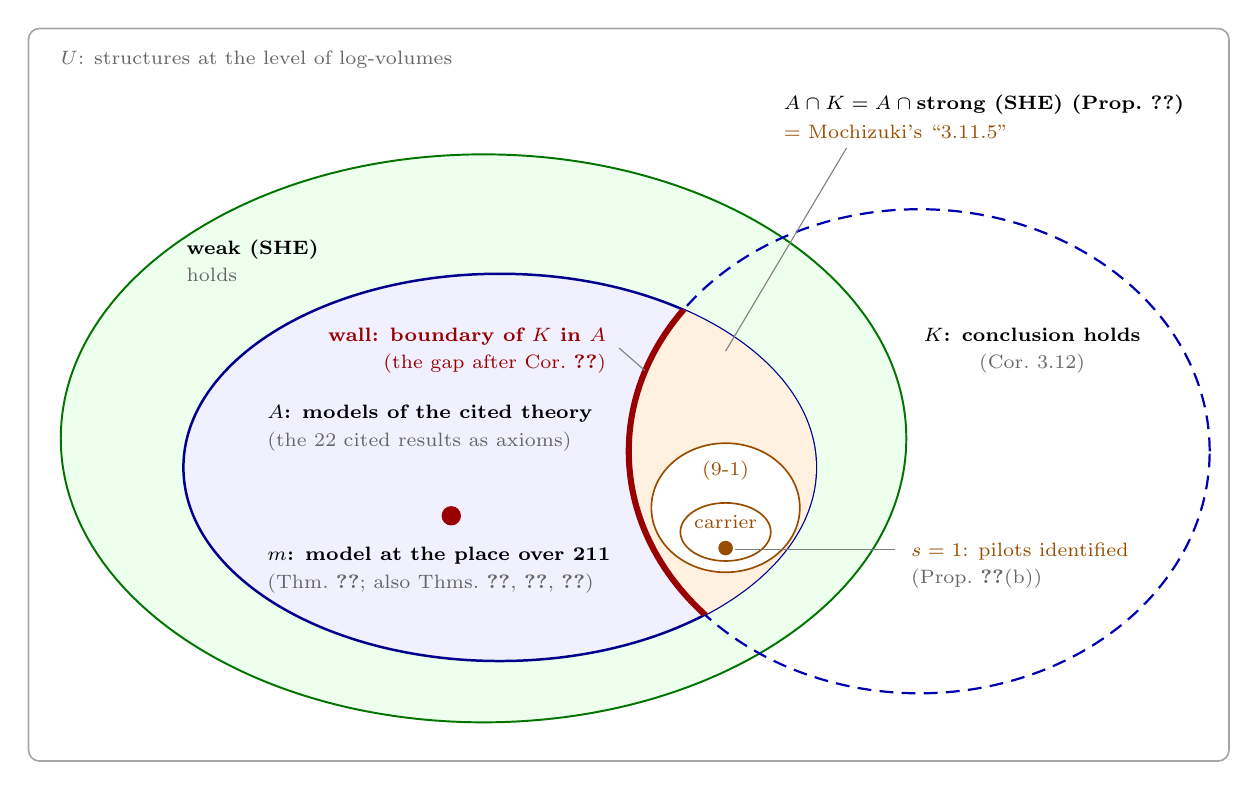
\begin{tikzpicture}[x=0.0205cm,y=0.0205cm,font=\scriptsize]
  % U
  \draw[black!35,line width=0.6pt,rounded corners=4pt] (8,8) rectangle (752,462);
  \node[anchor=base west,text=black!60] at (22,440) {$U$: structures at the level of log-volumes};
  % weak (SHE)
  \filldraw[fill=green!7,draw=green!45!black,line width=0.7pt] (290,208) ellipse [x radius=262,y radius=176];
  \node[anchor=base west,font=\scriptsize\bfseries] at (100,322) {weak (SHE)};
  \node[anchor=base west,text=black!60] at (100,305) {holds};
  % A
  \filldraw[fill=blue!6,draw=blue!55!black,line width=0.9pt] (300,190) ellipse [x radius=196,y radius=120];
  % A cap K
  \begin{scope}
    \clip (560,200) ellipse [x radius=180,y radius=150];
    \fill[orange!12] (300,190) ellipse [x radius=196,y radius=120];
  \end{scope}
  % K
  \draw[blue!70!black,line width=0.8pt,dash pattern=on 5pt off 3pt] (560,200) ellipse [x radius=180,y radius=150];
  % wall: boundary of K inside A
  \begin{scope}
    \clip (300,190) ellipse [x radius=196,y radius=120];
    \draw[red!60!black,line width=2.2pt] (560,200) ellipse [x radius=180,y radius=150];
  \end{scope}
  \node[anchor=base east,text=red!60!black,font=\scriptsize\bfseries] at (372,268) {wall: boundary of $K$ in $A$};
  \node[anchor=base east,text=red!60!black] at (372,251) {(the gap after Cor.~\ref{c:gap})};
  \draw[black!50,line width=0.4pt] (374,264) -- (390,250);
  \node[anchor=base west,font=\scriptsize\bfseries] at (150,220) {$A$: models of the cited theory};
  \node[anchor=base west,text=black!60] at (150,203) {(the 22 cited results as axioms)};
  \node[anchor=base,font=\scriptsize\bfseries] at (630,268) {$K$: conclusion holds};
  \node[anchor=base,text=black!60] at (630,251) {(Cor.~3.12)};
  % (9-1) and carrier
  \filldraw[fill=white,draw=orange!60!black,line width=0.6pt] (440,165) ellipse [x radius=46,y radius=40];
  \node[anchor=base,text=orange!60!black] at (440,185) {(9-1)};
  \filldraw[fill=white,draw=orange!60!black,line width=0.6pt] (440,150) ellipse [x radius=28,y radius=18];
  \node[anchor=base,text=orange!60!black] at (440,152) {carrier};
  \fill[orange!60!black] (440,140) circle [radius=4.5];
  \draw[black!50,line width=0.4pt] (446,139) -- (545,139);
  \node[anchor=base west,text=orange!60!black] at (549,135) {$s=1$: pilots identified};
  \node[anchor=base west,text=black!60] at (549,118) {(Prop.~\ref{p:horns}(b))};
  % A cap K callout
  \draw[black!50,line width=0.4pt] (515,388) -- (440,262);
  \node[anchor=base west,font=\scriptsize\bfseries] at (470,412) {$A\cap K=A\cap{}$strong (SHE) (Prop.~\ref{p:strong})};
  \node[anchor=base west,text=orange!60!black] at (470,394) {$=$ Mochizuki's ``3.11.5''};
  % m
  \fill[red!60!black] (270,160) circle [radius=6];
  \node[anchor=base west,font=\scriptsize\bfseries] at (150,132) {$m$: model at the place over 211};
  \node[anchor=base west,text=black!60] at (150,115) {(Thm.~\ref{t:main}; also Thms.~\ref{t:robust}, \ref{t:enlarged}, \ref{t:actual})};
\end{tikzpicture}
\caption{Each statement drawn as the class of structures in which it holds; the stronger
the statement, the smaller the class. Sizes and shapes are schematic, and the positions of
the points measure nothing. The exact relations are (a)--(e) below; no inclusion is claimed
that is not listed there. The reconstruction content of Theorem~3.11 (Kummer classes of
theta values, cyclotomic rigidity) does not appear at this level: Step (xi-b) forgets it.}\label{fig:venn}
\end{figure}

\begin{enumerate}[label=(\alph*),leftmargin=2.2em]
\item \Pmark{} $A$ lies inside the class of weak (SHE): weak (SHE) holds in every model of
  the cited theory (Proposition~\ref{p:weak}).
\item \Pmark{} $A$ does not lie inside $K$: $A$ contains a model $m$ in which the
  conclusion fails (Theorem~\ref{t:main}); the same holds after adding places, after
  enlarging the container, and when the model is built on actual local objects
  (Theorems~\ref{t:robust}, \ref{t:enlarged} and~\ref{t:actual}).
\item \Pmark{} Inside $A$, the class $K$ coincides with the class of strong (SHE) in the
  value reading; the class of the carrier reading lies inside that of (9-1), and that of
  (9-1) inside $K$ (Proposition~\ref{p:strong}).
\item \Pmark{} A structure in which the images of the two pilots are identified satisfies
  the carrier reading and lies in $K$, and its degree scale is then $s=1$; conversely, $s=1$
  together with an image of the $\Theta$-pilot of nonzero measure gives $K$
  (Proposition~\ref{p:horns}(b)(c)).
\item \Hmark{} The statement ``3.11.5'' (Theorem~3.11 together with Remark~3.9.5) that
  Mochizuki isolates in his report on formalization \cite[\S4]{Form} corresponds to the
  intersection of $A$ with strong (SHE), that is, to $A\cap K$, and implies the conclusion
  (\S\ref{s:rel}). Whether a model in $A$ crosses the boundary of $K$ is whether the gap
  $\vol(q)-\vol(H)$ of the remark following Corollary~\ref{c:gap} is covered; this is the
  position of the inequality in \texttt{xi\_iff} of \cite{lana}.
\end{enumerate}

\Smark{} In Step (xi-b) the author states that he takes the point of view of ``temporarily
forgetting'' that the multiradial construction algorithm of \cite[Thm.~3.11]{IUT3}
involves $\Theta$-pilot objects, theta functions/values and mono-theta environments
(\S\ref{s:step}). \Hmark{} Hence the reconstruction content of Theorem~3.11 does not appear
at the level of Figure~\ref{fig:venn}: within Step (xi), strengthening it does not push the
model $m$ out of $A$, since Step (xi) reads only (IPL), (SHE) and (APT). This does not
exclude that the construction itself supplies the missing statement (see \emph{Not claimed}
above).

\section{The step}\label{s:step}

\Smark{} \cite[Cor.~3.12]{IUT3} asserts that $-|\log(\Thbb)|\ge-|\log(\qbb)|$, where
$-|\log(\qbb)|$ is the log-volume of the $q$-pilot object and $-|\log(\Thbb)|$ is the
procession-normalized log-volume of the holomorphic hull of the union of the possible
images of the $\Theta$-pilot object, subject to the indeterminacies (Ind1), (Ind2),
(Ind3). The inequality is obtained in Step (xi) of the proof; the last step, (xii),
comments on the role of the global realified Frobenioids (\S\ref{s:omitted}). In (xi-b)
the author writes (here and below, emphasis in the original is omitted):
\begin{quote}
Also, in this context, we observe that, although the multiradial construction algorithm of
Theorem 3.11 in fact involves the $\Theta$-pilot object at $(0,0)$, in the present
discussion of Step (xi), we shall only be concerned with qualitative logical
aspects/consequences of this construction algorithm, i.e., with the
\begin{itemize}[label=$\cdot$,leftmargin=1.5em,itemsep=0pt,topsep=2pt]
\item input prime-strip link (IPL),
\item simultaneous holomorphic expressibility (SHE), and
\item algorithmic parallel transport (APT)
\end{itemize}
properties discussed in Remark 3.11.1, (iii), (iv), (v). That is to say, we shall take the
point of view of ``temporarily forgetting'' --- cf. the discussion of hidden internal
structures (HIS) in Remark 3.11.1, (iv) --- the fact that the multiradial construction
algorithm of Theorem 3.11 in fact involves $\Theta$-pilot objects, theta functions/values,
mono-theta environments. Alternatively, in the discussion to follow, we shall, roughly
speaking, think of the multiradial construction algorithm of Theorem 3.11 as ``some''
algorithm that transforms a certain type of input data into a certain type of output data
and, moreover, satisfies certain properties (IPL) and (SHE).
\end{quote}
Step (xi-f) reads, in part:
\begin{quote}
Thus, we conclude from (xi-e) that the construction of the subset
$\mathbb R_{\le-|\log(\Thbb)|}\subseteq\mathbb R$ of possible pilot-object
log-volumes of output data is subject to the condition that this construction of output
data possibilities constitutes, in particular, a construction [perhaps only up to some
sort of ``approximation'', as a result of various indeterminacies] of the pilot-object
log-volume of the input data \textup{(}$\mathcal F^{\Vdash\blacktriangleright\times\mu}$-\textup{)}prime-strip,
namely, $-|\log(\qbb)|\in\mathbb R$.
\end{quote}
The inclusion $-|\log(\qbb)|\in\mathbb R_{\le-|\log(\Thbb)|}$ is then the conclusion.

\Smark{} We read every citation in the statement and the proof of \cite[Cor.~3.12]{IUT3}
and classified its role (Table~\ref{tab:inv}). The statement, which cites the definitions
of the two log-volumes, is counted together with the proof.
\begin{table}[!tbp]
\centering
\begin{tabular}{lrp{0.5\textwidth}}
\toprule
role in the proof & targets & examples\\
\midrule
definition (A) & 5 & \cite[Def.~3.1]{IUT1}, \cite[Cor.~4.10]{IUT2}; Def.~2.4, Rem.~3.1.1, Def.~3.8\\
definition and premise (A+B) & 2 & Prop.~3.9, Rem.~3.9.5\\
premise (B) & 15 & Thm.~1.5, Thm.~3.11, Rem.~3.11.1, and twelve further remarks\\
background & 31 & \\
comments and figures & 8 & Rem.~3.6.2, \cite{IUT4}, Figs.~3.6--3.8\\
\bottomrule
\end{tabular}
\caption{The 61 targets cited in the statement and proof of
\cite[Cor.~3.12]{IUT3}.}\label{tab:inv}
\end{table}
Unless otherwise indicated, numbered items in the table are those of \cite{IUT3}.
\cite[Prop.~3.5(ii)]{IUT3}, which we also use, is not cited by the proof directly but by
\cite[Thm.~3.11(ii)]{IUT3}, in the passage quoted in Remark~\ref{r:strength}.
Theorem~3.11 is stated without (IPL) and (SHE); the two properties are introduced in
\cite[Rem.~3.11.1(iii)]{IUT3} (``IPL'' is mentioned before, in a forward reference in
\cite[Rem.~3.9.5(ix)]{IUT3}), where (SHE) is said to correspond to the closed loop of
\cite[Rem.~3.9.5(viii)(ix)]{IUT3} (\S\ref{s:layer}). \Smark{} Steps (xi-e) and (xi-f)
invoke no numbered result as a premise: (xi-e) names the multiradial construction algorithm
of Theorem~3.11, whose output it describes, and (xi-f) the statement of Corollary~3.12.

\Hmark{} The passage from (xi-b) fixes the level of abstraction of this note. The axioms
below record what the cited results say about log-volumes, and the readings of (SHE)
record what Step (xi) may take from that property; the internal structure that (xi-b)
sets aside is not used.

\section{The cited results as axioms}\label{s:axioms}

\begin{definition}[packets]\label{d:packet}
A \emph{packet system} consists of $\ell^*\ge1$; a finite set of places $v$; for each
place $v$ a finite set $V_v$ (the direct summands) and, for each $\beta\in V_v$, two groups
$A_{v,\beta}$ (automorphisms of a component of a prime-strip) and $\Ism_{v,\beta}$, the
elements of the latter having order dividing $2$ when $v$ is archimedean; and for each
place $v$ and stage $j\in\{0,\dots,\ell^*\}$: a locally compact abelian topological group
$P_{v,j}$ with a regular Haar measure $\mu_{v,j}$; a compact subset $\cO_{v,j}$ with
nonempty interior (the mono-analytic integral structure
\cite[Prop.~3.2(ii), Rem.~3.9.1(i)]{IUT3}); a weight $w_{v,j}>0$ and a constant $a_{v,j}$
(accounting for the discrepancy between the mono-analytic and the local holomorphic
integral structures discussed in \cite[Rem.~3.9.1]{IUT3}); and three actions on $P_{v,j}$
by automorphisms of topological groups preserving $\cO_{v,j}$, each respecting identity
and composition: of the permutations of the labels $\{0,\dots,j\}$, of the families
$(g_{\alpha,\beta})$ with $g_{\alpha,\beta}\in A_{v,\beta}$ indexed by labels $\alpha$ and
summands $\beta$, and of the families of elements of the groups $\Ism_{v,\beta}$ indexed in
the same way. (Ind1) sends a region to its image under a family of automorphisms of
prime-strips composed with a permutation of the labels at each stage, the permutation being
the same at all places; (Ind2) sends it to its image under a family of copies of $\Ism$.
A \emph{region} is a family $x=(x_{v,j})$ of subsets $x_{v,j}\subseteq P_{v,j}$; it has
\emph{nonzero measure} if $\mu_{v,j}(x_{v,j})\ne0$ for all $v$ and $j$. Its
\emph{normalized log-volume} is
\[
\vol(x)=\sum_v\frac1{\ell^*}\sum_{j=1}^{\ell^*}
\Bigl(w_{v,j}\bigl(\log\mu_{v,j}(x_{v,j})-\log\mu_{v,j}(\cO_{v,j})\bigr)+a_{v,j}\Bigr).
\]
We write $x\le y$ if $x_{v,j}\subseteq y_{v,j}$ for all $v,j$.
\end{definition}

This is \cite[Prop.~3.9(i)]{IUT3} with the procession normalization of
\cite[Rem.~3.1.1]{IUT3}: an average over the labels $j\in\mathbb F_\ell^*$ and a sum
over places. By \cite[Prop.~3.9(iii)]{IUT3} it computes arithmetic degrees. Because the
automorphisms preserve $\cO_{v,j}$, they preserve the Haar measure, and hence $\vol$.

\begin{definition}[cited theory]\label{d:cited}
A \emph{cited theory} is a packet system with regions $\theta$ (image of the
$\Theta$-pilot), $q$ (image of the $q$-pilot), $C$ (the container), $H$ (the hull), a set
$\Poss$ of regions (the possible images), a class $\Lambda$ of subsets of the $P_{v,j}$
(in the source, the sets $\lambda\cdot\tO$ for the ring of integers $\tO$ of the packet; see
Remark~\ref{r:strength}), and a real number $s$ (the degree scale), such that:
\begin{enumerate}[label=(C\arabic*),leftmargin=2.8em]
\item\label{c:theta} $\theta\in\Poss$. \hfill\cite[Def.~3.8(i), Thm.~3.11(i)]{IUT3}
\item\label{c:ind12} $\Poss$ is closed under (Ind1) and (Ind2) of
  Definition~\ref{d:packet}. \hfill\cite[Thm.~3.11(i)]{IUT3}
\item\label{c:ind3} Every $x\in\Poss$ satisfies $x\le C\le\cO$; and if $x\in\Poss$ and
  $x\le y\le C$ then $y\in\Poss$. \hfill (Ind3), \cite[Thm.~3.11(ii), Prop.~3.5(ii)]{IUT3}
\item\label{c:hull} $H_{v,j}\in\Lambda$ for all $v,j$; $x\le H$ for all $x\in\Poss$;
  $H\le T$ for every region $T$ with all $T_{v,j}\in\Lambda$ and $x\le T$ for all
  $x\in\Poss$; and $H\le\cO$. \hfill\cite[Rem.~3.9.5(i)]{IUT3}
\item\label{c:q} $q\le\cO$, every $\mu_{v,j}(q_{v,j})\ne0$, and $\vol(q)<0$.
  \hfill\cite[Def.~3.1(b)]{IUT1}
\item\label{c:link} $s>0$ and $\vol(q)=s\cdot\vol(\theta)$.
  \hfill\cite[Def.~3.8(ii)]{IUT3}; see Remark~\ref{r:strength}
\item\label{c:ipl} For every $x\in\Poss$ there is $c>0$ with $\vol(q)=c\cdot\vol(x)$.
  \hfill (IPL), \cite[Rem.~3.11.1(iii)]{IUT3}
\end{enumerate}
Put $-|\log(\Thbb)|:=\vol(H)$ and $-|\log(\qbb)|:=\vol(q)$. The \emph{conclusion} is
$\vol(q)\le\vol(H)$.
\end{definition}

\begin{remark}[on the strength of the axioms]\label{r:strength}
\Smark{} \ref{c:ind3}: \cite[Thm.~3.11(ii)]{IUT3} imposes the upper
semi-compatibility (Ind3) on the Kummer isomorphisms of tensor packets of log-shells.
For the splitting monoids (theta values) and the copies of $F_{\mathrm{mod}}$ it states
instead that they are mutually compatible along the log-links, ``in the sense that the
only portions [\dots] that are possibly related to one another via the log-links consist
of roots of unity [\dots] multiplication by which corresponds, via the log-link, to an
`addition by zero' indeterminacy, i.e., to no indeterminacy!'' \Hmark{} Thus the possible images
lie in the log-shell packet multiplied by the theta values $\qbb^{\,j^2}$, and this is our
$C$. We take the \emph{largest} reading: everything between an image and $C$ is possible.
A smaller set of possible images can only shrink the hull
(Proposition~\ref{p:horns}(a), Proposition~\ref{p:restrict}).

\Smark{} \ref{c:hull}: \cite[Rem.~3.9.5(i)]{IUT3} defines the holomorphic hull of a
relatively compact $U$ as ``the smallest subset of the form'' $\lambda\cdot\tO$ that
contains $U$, where $\tO$ is the ring of integers of the tensor packet, which is a direct
sum of fields, and each component of $\lambda$ is nonzero. This is the holomorphic
integral structure; $\cO$ denotes the mono-analytic one.

\Smark{} \ref{c:link}: the $\Theta_{\mathrm{LGP}}$-link sends the $\Theta$-pilot to the
$q$-pilot, and an isomorphism of Frobenioids preserves only isomorphism classes of
objects \cite[Rem.~3.6.2(i)]{IUT3}; the arithmetic degree is determined up to a positive
real multiple \cite[Cor.~4.10(v)]{IUT2}. Neither statement is a premise of the proof: the
proof cites \cite[Rem.~3.6.2(i)]{IUT3} only in Step (xii), where it explains why global
realified Frobenioids are needed (Table~\ref{tab:inv} counts it among the comments), and
the statement of \cite[Cor.~3.12]{IUT3} and Step (x) of the proof cite
\cite[Cor.~4.10]{IUT2} only for part (i). \Hmark{} We keep $s$ free and use the
two statements only to justify this; by Proposition~\ref{p:horns}(c), fixing $s=1$ would
give the conclusion whenever $\theta$ has nonzero measure. \Smark{} That a positive
rescaling of one side alone cannot be controlled by comparisons that are invariant under it
is \cite[Cor.~9.2]{Pajo}. \Hmark{} Here the freedom has a source, namely the two
statements just cited.

\ref{c:ipl} is the degree-level content of (IPL): the output is related to the input by a
full poly-isomorphism, which on degrees gives a positive multiple and nothing more.
\end{remark}

\begin{definition}[readings of (SHE)]\label{d:she}
For a cited theory:
\begin{itemize}[leftmargin=2em]
\item \emph{weak (SHE)}: there is a map $\mathrm{alg}$ from regions to sets of regions
  with $\Poss=\mathrm{alg}(C)$ and $y\le c$ whenever $y\in\mathrm{alg}(c)$. (The possible
  images are computed from the container, which is common to both sides.)
\item \emph{strong (SHE), carrier reading}: $q\in\Poss$.
\item \emph{strong (SHE), value reading}: $\vol(q)\in\mathbb R_{\le\vol(H)}$.
\item \emph{(9-1)} \cite[\S\S9.2--9.3]{LANA}, in the reading explained below: there is
  $x\in\Poss$ of nonzero measure with $\vol(x)=\vol(q)$.
\end{itemize}
\end{definition}

\Hmark{} \cite[Rem.~3.11.1(iii)]{IUT3} describes (SHE) as the property that the output
data and its construction are expressible in terms valid simultaneously for the
arithmetic holomorphic structures on both sides. We do not decide between the readings.
The value reading is the conclusion rewritten in the language of (xi-d); the carrier
reading is the closed loop of \cite[Rem.~3.9.5(viii)(ix)]{IUT3} taken literally.

\Smark{} On (9-1): \cite[\S9.2]{LANA} constructs two isomorphisms of pointed real vector
spaces $\eta^q,\eta^{\mathrm{anab}}_S:\mathbb R^{\mathrm{val}}\to\mathbb R^{\mathrm{ss}}$,
where $\mathbb R^{\mathrm{ss}}$ consists of the adelic measurable subsets of a large-volume
container modulo equality of volume; $\eta^{\mathrm{anab}}_S$ sends the pilot to the class
of $\mathrm{LGP}\cdot S$, and $\eta^q$ sends it to the class of
$\{q_{\underline v}\,\mathcal O_{\underline v}\}$, where $q_{\underline v}$ is the
$q$-parameter and $\mathcal O_{\underline v}$ the ring of integers. The $q$-pilot of
\cite[\S4.2(c)]{LANA} is built from a $2\ell$-th root of $q_{\underline v}$, and
\cite[\S9.3]{LANA} reads (9-1) as saying that ``at the level of degree (log-volume), the
rigidified $q$-pilot is represented in the output regions''. \Hmark{} We follow this
reading: we take the pilot of $\eta^q$ to be the class of the $q$-pilot region, and the
regions $\mathrm{LGP}\cdot S$, for the $S$ that \cite[\S9.2]{LANA} calls suitable, to be the
possible images. Two isomorphisms of pointed one-dimensional real vector spaces agree if
and only if they agree on the pilot, so, under these identifications,
$\eta^q=\eta^{\mathrm{anab}}_S$ for some suitable $S$ if and only if some possible image
has the log-volume of the $q$-pilot; this is the fourth item above. Read literally, with
$q_{\underline v}$ in place of its $2\ell$-th root, the region
$q_{\underline v}\mathcal O_{\underline v}$ has, at each bad place, $2\ell$ times the
log-volume of the $q$-pilot region there, and (9-1) would compare the possible images with
that multiple.

\begin{proposition}\label{p:weak}
\Pmark{} Weak (SHE) holds in every cited theory: take $\mathrm{alg}(c)$ to be the set of
possible images $y$ with $y\le c$; then $\mathrm{alg}(C)=\Poss$ by \ref{c:ind3}.
\end{proposition}

So the axioms together with weak (SHE) have the same models as the axioms alone. We keep
weak (SHE) in view because it is the reading of (SHE) that the cited statements support:
the possible images are computed from the common container. It does not close the gap.

\begin{proposition}\label{p:strong}
\Pmark{} In a cited theory: the value reading is equivalent to the conclusion; the
carrier reading implies (9-1); (9-1) implies the conclusion.
\end{proposition}

\begin{proof}
The first is the definition of $\mathbb R_{\le a}$. The second takes $x=q$. For the third,
$x\le H\le\cO$ by \ref{c:hull}, and on each $P_{v,j}$ the function
$A\mapsto w(\log\mu(A)-\log\mu(\cO))$ is monotone for $A\subseteq\cO$ of nonzero
measure; summing gives $\vol(q)=\vol(x)\le\vol(H)$.
\end{proof}

\begin{remark}[the approximation in (xi-f)]\label{r:approx}
Step (xi-f) allows the construction of $-|\log(\qbb)|$ to hold ``perhaps only up to some
sort of `approximation'\,''. Since the set of possible values is a closed half-line,
approximate membership from below is the same as membership: $\vol(q)\le\vol(H)+\varepsilon$
for every $\varepsilon>0$ if and only if $\vol(q)\le\vol(H)$. This is
\cite[Lemma~4.1]{Higuchi}. \Pmark{} Consequently the approximate form fails in every model
below in which the conclusion fails.
\end{remark}

\section{A model at one place}\label{s:model}

\Smark{} The initial $\Theta$-datum of \cite[Thm.~1]{First} has $\ell=7$, so $\ell^*=3$.
Above the split prime $211$ it has one selected bad place and one good place; at the bad
place the ramification index is $e_{\mathrm b}=105$ and
$\mathrm{ord}_{211}(\qbb_{\mathrm b})=29/7$. The model of this section keeps $\ell$ and
the valuation, and replaces the completion at the bad place by $\Qp{211}$; \S\ref{s:robust}
enlarges the container at that place by a fixed factor, and \S\ref{s:actual} builds the
model from the actual local objects at a finite extension of $\Qp p$ that carries a theta
datum.

\begin{definition}\label{d:model}
Let $P_j=\Qp{211}^{\,j+1}$ with the product Haar measure normalized by
$\mu(\mathbb Z_{211}^{\,j+1})=1$, let $\cO_j=\mathbb Z_{211}^{\,j+1}$, $w_j=1/(7(j+1))$
and $a_j=0$. Let the automorphisms be the coordinate permutations and the coordinatewise
multiplications by $\mathbb Z_{211}^\times$. Let $B(j,k)=(211^k\mathbb Z_{211})^{j+1}$
and $\Lambda=\{B(j,k):k\ge0\}$. Put
\[
\theta_j=C_j=H_j=B(j,29j^2),\qquad q_j=B(j,29),\qquad \Poss=\{\theta\},\qquad s=3/14.
\]
\end{definition}

The weight $1/(j+1)$ is the packet normalization; the constant factor $1/7$ makes
$\vol(q)=-\mathrm{ord}_{211}(\qbb)\log211$. No statement below changes if all weights are
multiplied by the same positive constant.

Here $\cO_j$ is also the ring of integers of $P_j$. The class $\Lambda$ consists of the
sets $\lambda\cdot\cO_j$ for which the components of $\lambda$ all have the same
nonnegative valuation; it is smaller than the class of
\cite[Rem.~3.9.5(i)]{IUT3}. This does not matter here: $C=\theta$ is itself a possible
image and lies in $\Lambda$, so any region of the larger class containing the possible
images contains $C$, and the smallest one is $C$ in either class. (The model of
\S\ref{s:actual} uses the full class.)

The log-shell of a nonarchimedean local field $k$ with ring of integers $\cO_k$ is
$I_k=(p^*)^{-1}\log_k(\cO_k^\times)$,
with $p^*=p$ for odd $p$ and $p^*=p^2$ for $p=2$ \cite[Rem.~1.2.2(i)]{IUT3}. For $k=\Qp{211}$ this is
$211^{-1}\cdot211\,\mathbb Z_{211}=\mathbb Z_{211}$, so (Ind3) does not enlarge anything
on this carrier and $C=\qbb^{\,j^2}\cdot\cO$ is the possible image itself. For the actual
completion $K$ at the bad place, with $e=105<210=p-1$, the logarithm maps $1+\mathfrak m_K$
onto $\mathfrak m_K$ and $K$ contains no nontrivial $p$-power roots of unity, so
$I_K=p^{-1}\mathfrak m_K\supsetneq\cO_K$. The container is then larger than the image of the
$\Theta$-pilot, by a factor that does not depend on the Tate parameter.
Theorem~\ref{t:enlarged} below
covers enlargements by $211^{c}$; Theorem~\ref{t:actual} treats the actual objects.

\begin{lemma}\label{l:vols}
\Pmark{} Put $u=-\frac{29}{7}\log211<0$. At every stage $j$,
$w_j\bigl(\log\mu(B(j,29m))-\log\mu(\cO_j)\bigr)=m\,u$. Hence $\vol(q)=u$ and
$\vol(\theta)=\frac{1+4+9}{3}\,u=\frac{14}{3}\,u$.
\end{lemma}

\begin{proof}
$\mu(B(j,k))=211^{-k(j+1)}$, so $w_j\log\mu(B(j,29m))=-\frac{29m}{7}\log211$.
\end{proof}

Note that $14/3=\ell(\ell+1)/12$ for $\ell=7$, the familiar factor.  Its reciprocal
$12/(\ell(\ell+1))$ is the constant $\chi$ compared in \cite{Fifth}, where it is identified
as the ratio of the stage-one coefficient $1/(2\ell)$ to the mean of $j^2/(2\ell)$.

\begin{theorem}\label{t:main}
\Pmark{} The data of Definition~\ref{d:model} form a cited theory in which the conclusion
fails: $\vol(q)=u>\frac{14}3u=\vol(H)$. Hence none of the conclusion, the carrier reading,
the value reading, or (9-1) follows from the axioms of a cited theory, even together with
weak (SHE).
\end{theorem}

\begin{proof}
\ref{c:theta}, \ref{c:hull}, \ref{c:q} are immediate: $\theta$ is the only possible image,
it is a box $B(j,29j^2)\in\Lambda$, so it is the smallest region of $\Lambda$ containing
the possible images, and $\vol(q)=u<0$. \ref{c:ind12}: permutations and multiplication by
units preserve $B(j,k)$. \ref{c:ind3}: $x\le y\le C=\theta$ forces $y=\theta$.
\ref{c:link}: $u=\frac3{14}\cdot\frac{14}3u$. \ref{c:ipl} with $c=3/14$. The conclusion $u\le\frac{14}3u$ is false because $u<0$; the
readings and (9-1) fail by Proposition~\ref{p:strong}.
\end{proof}

\begin{corollary}[where the gap lies]\label{c:gap}
\Pmark{} Weak (SHE) holds in every cited theory; in every cited theory the value reading is
equivalent to the conclusion; and neither the carrier reading nor the value reading holds
in every cited theory.
\end{corollary}

\begin{proof}
Propositions~\ref{p:weak} and~\ref{p:strong}, and Theorem~\ref{t:main}.
\end{proof}

\Hmark{} So the whole distance between the axioms and the conclusion lies between the
weak and the strong readings of (SHE). This is partly a matter of definition, since the
value reading is the conclusion rewritten; the content is that the weak reading follows
from the axioms and the strong readings do not. In the source, the passage between the two
readings is the passage from (xi-e), which invokes (SHE), to (xi-f), which draws the
membership. \Smark{} Higuchi locates the same passage for his qualitative package
\cite{Higuchi}. \Hmark{} The corollary shows that the log-volume content of the cited
results does not close it.

\begin{remark}
The scale $s=3/14=12/(\ell(\ell+1))$ is not chosen: \ref{c:link} forces it from the two
volumes, which are determined by the valuation of the datum and the Haar measure. The gap
$\vol(q)-\vol(H)=\frac{11}3|u|$ is what (Ind3) would have to cover.
\end{remark}

\begin{remark}\label{r:weakaxioms}
\ref{c:link} and \ref{c:ipl} can be satisfied, by choosing $s$ and the constants $c$,
whenever the volumes involved are negative: they fix a positive ratio and nothing more. This is the content of (IPL) at the level of degrees, and
it is why the degree scale is a parameter of the model rather than a constraint on it.
\end{remark}

\section{Any number of places}\label{s:robust}

A cited theory over several places is defined in the same way, with regions indexed by
places and $\vol$ summed over them; $\ell^*$ is common to all places. Each place carries its
own packet system, so the possible images are required to be closed under (Ind1) and (Ind2)
chosen independently at the different places. For the label permutations of (Ind1) this is
the stronger requirement; the automorphisms of (Ind2) are chosen place by place in either
case. An \emph{extra
place} is any packet system with $\ell^*=3$ together with a region $q^{\mathrm{ex}}\le\cO$
of nonzero measure. At an extra place we take the $\Theta$-side image, the container,
the hull and the only possible image to be the whole integral structure $\cO$, and
$\Lambda=\{\cO\}$; since $\cO$ is then the only possible image, $H=\cO$ is also the
smallest member of any class that contains $\cO$. This is the largest enlargement that
(Ind3) permits, and it makes the hull as large as possible.

At the place over $211$ we multiply the valuations of both pilots by $N$:
$\theta^{(N)}_j=B(j,29Nj^2)$ and $q^{(N)}_j=B(j,29N)$. This is what replacing the Tate
parameter by its $N$-th power would do; it is a family of data, not a remark of the
source.
(\cite[Rem.~3.11.1(ii)]{IUT3} replaces only the $q$-pilot by the $q^\lambda$-pilot, which
makes the conclusion weaker, not stronger.) The data of this family are not claimed to come
from elliptic curves: for actual curves the contributions of the other places need not stay
fixed as the valuation of the Tate parameter grows.

\begin{theorem}\label{t:robust}
\Pmark{} For every finite family of extra places there is $N$ such that the resulting
data form a cited theory over all places in which the conclusion fails. In particular this holds with two extra places: one over $\Qp5$ (packets $\Qp5$ at
every stage, $\cO=\mathbb Z_5$, $q$-component $5\mathbb Z_5$), and one archimedean place
(packets $\mathbb R^{j+1}$ with Lebesgue measure, $\cO$ the closed unit ball, weights
$1/(j+1)$, $q$-component the closed ball of radius $1/2$).
\end{theorem}

\begin{proof}[Sketch]
Let $A=\sum\vol(\cO^{\mathrm{ex}})$ and $B=\sum\vol(q^{\mathrm{ex}})\le A$ over the extra
places. The total volumes are $N\frac{14}3u+A$ and $Nu+B$. The conclusion would require
$\frac{11}3N|u|\le A-B$, which fails for large $N$. The axioms are checked place by
place; the only new point is that the automorphisms preserve $\cO$.
\end{proof}

We now separate the image of the $\Theta$-pilot from the container at the bad place: for
a fixed integer $c\ge0$ let
\[
\theta^{(N)}_j=B(j,29Nj^2),\qquad C^{(N,c)}_j=B\bigl(j,\max(29Nj^2-c,0)\bigr),
\]
(for $c\le29N$ the maximum is $29Nj^2-c$ at the stages $j\ge1$, and $0$ at the stage
$j=0$, which does not enter $\vol$)
and let $\Poss$ consist of the regions $x$ with $\theta^{(N)}\le x\le C^{(N,c)}$ at the bad
place and $x=\cO$ at the extra places, so that the possible images form the whole interval
between the image and the container, and the hull is $C^{(N,c)}$. The container exceeds
the image in normalized log-volume by $\frac c7\log211$, independently of $N$.

\begin{theorem}\label{t:enlarged}
\Pmark{} For every integer $c\ge0$ and every finite family of extra places there is $N$ with
$c\le29N$ such that these data form a cited theory over all places in which the conclusion
fails. For $c>0$ the image of the $\Theta$-pilot and the container are
different regions.
\end{theorem}

\begin{proof}[Sketch]
The total volumes are $N\frac{14}3u+\frac c7\log211+A$ for the hull and $Nu+B$ for the
$q$-pilot. The conclusion would require $\frac{11}3N|u|\le\frac c7\log211+A-B$, which
fails for large $N$. Closure under (Ind1), (Ind2) holds because the automorphisms fix both
ends of the interval and preserve inclusions; every possible image contains
$\theta^{(N)}$ and so has nonzero measure.
\end{proof}

\section{The model on the actual local objects}\label{s:actual}

The models above replace the completion at the bad place by $\Qp{211}$ and let the
indeterminacies act by coordinate permutations and units. We now build the model from the
actual local objects at a finite extension of $\Qp p$, ramified or not, that carries a theta
datum (Definition~\ref{d:thetadatum}).

\subsection{Packets and the integral structure}\label{s:packets}

Let $p$ be a prime and $L$ a finite extension of $\Qp p$, with ring of integers $R$,
ramification index $e$ and a uniformizer $\pi$. For $j\in\{0,1,2,3\}$ let $I=\{0,\dots,j\}$,
let $P_j=L^{\otimes I}$ be the tensor product over $\Qp p$ of $j+1$ copies of $L$, and let
$\tI\subseteq P_j$ be the integral closure of $\mathbb Z_p$ (the ring of integers $\tO$ of
the packet). Let $\log_p(R^\times)\subseteq L$
be the image under $\log_p$ of the principal units $1+\mathfrak m_R$; it is also the image
of $R^\times$, since $R^\times$ is the product of $1+\mathfrak m_R$ and the roots of unity
of order prime to $p$, on which $\log_p$ vanishes (a standard fact, not formalized). Let
$\log_p(R_I^\times)\subseteq P_j$ be the $\mathbb Z_p$-module generated by the pure tensors
of elements of $\log_p(R^\times)$ \cite[Prop.~1.2]{IUT4}; on each factor
$\log_p(R^\times)=p^*\cdot I_L$, where $I_L$ is the log-shell of \S\ref{s:model}. The constants $\mathfrak d_I$, $a_I$, $b_I$ are those of
\cite[Prop.~1.1, 1.2]{IUT4}, computed from the actual different and ramification of $L$.
For $x\in L$ we write $x_{(1)}=x\otimes1\otimes\dots\otimes1\in P_j$, and for
$\lambda=k/e$ we write $p^\lambda\cdot\tI$ for $(\pi^k)_{(1)}\cdot\tI$.

\begin{lemma}\label{l:shell}
\Pmark{} $\log_p(R_I^\times)$ is a compact open subgroup of $P_j$. For every
$\mathbb Q_p$-linear automorphism $\phi$ of $P_j$ with $\phi(\log_p(R_I^\times))=
\log_p(R_I^\times)$ and every $\lambda\in e^{-1}\mathbb Z$,
\[
\phi\bigl(p^\lambda\tI\bigr)\subseteq p^{\lfloor\lambda-\mathfrak d_I-a_I\rfloor}
\log_p(R_I^\times)\subseteq p^{\lfloor\lambda-\mathfrak d_I-a_I\rfloor}\cdot
\pi_I^{-b}\cdot\tI,
\]
where $\pi_I^{-b}$ is a pure tensor of powers of $\pi$ of total order $-b_I$
\cite[Prop.~1.2(ii)]{IUT4}.
\end{lemma}

We take the packet system with one place, $\ell^*=3$, $P_j$ as above,
$\cO_j=\log_p(R_I^\times)$, the Haar measure $\mu_j$ with $\mu_j(\tI)=1$, the weight
$w_j=1/[P_j:\Qp p]$ and the adjustment $a_j=w_j\log\mu_j(\cO_j)$. \Smark{} By
\cite[Rem.~3.9.1(i)]{IUT3} the mono-analytic integral structure is the tensor product of
the log-shells $I_L$, which differs from $\cO_j$ by the scalar $(p^*)^{j+1}$; and
\cite[Prop.~1.4(i)]{IUT4} normalizes log-volumes on such tensor products so that
$\mu^{\log}(\tI)=0$ and $\mu^{\log}(p\cdot\tI)=-\log p$.

\begin{lemma}\label{l:normalization}
\Pmark{} For every region $A\subseteq P_j$,
$w_j\bigl(\log\mu_j(A)-\log\mu_j(\cO_j)\bigr)+a_j=w_j\log\mu_j(A)$. Hence the packet
log-volume is the one normalized as in \cite[Prop.~1.4(i)]{IUT4}.
\end{lemma}

The identity is algebraic, and holds for any compact open choice of $\cO_j$ with $a_j$
defined in the same way; in particular it holds for the tensor product of the log-shells
itself.

The indeterminacies act as follows. A permutation $\sigma$ of the labels $I$ permutes the
tensor factors. An automorphism of prime-strips at a label, and a copy of $\Ism$ at a
label, act on the corresponding factor through a $\mathbb Z_p$-linear automorphism $g$ of
the log-shell $I_L$, extended $\Qp p$-linearly to $L$; the copies at different labels are
independent. We let $g$ run over \emph{all} $\mathbb Z_p$-linear automorphisms of $I_L$.
\Smark{} \cite[Thm.~3.11(i)]{IUT3} describes (Ind2) as induced ``by the action of
independent copies of $\Ism$ [\dots] on each of the direct summands of the $j+1$ factors
appearing in the tensor product''. By \cite[Prop.~1.2(vi)]{IUT3} the mono-analytic
log-shell is constructed by a functorial algorithm from the $\mathcal D^{\vdash}$-prime-strip,
and the $\Ism$-orbit of isomorphisms constructed there is compatible with the log-shells and
their log-volumes; so the indeterminacies of (Ind1) and (Ind2) act on each factor through
automorphisms of the log-shell. \Hmark{} We do not construct the maps from the groups of the
source to $\Aut_{\mathbb Z_p}(I_L)$; closure of the possible images under the full group
implies closure under their images.

\begin{lemma}\label{l:actions}
\Pmark{} These actions satisfy the group laws, preserve $\log_p(R_I^\times)$, and hence
preserve $\mu_j$. The copies of $\Ism$ in (Ind2), and the automorphisms of prime-strips in
(Ind1), act nontrivially for every $L$: multiplication by $-1$ on the log-shell sends
$1\in P_0$ to $-1$. If $L\ne\Qp p$, the label permutations in (Ind1) act nontrivially as
well: for $\alpha\in L\setminus\Qp p$, the transposition of the two labels of $P_1$ sends
$1\otimes\alpha$ to $\alpha\otimes1\ne1\otimes\alpha$; the $\Qp p$-linear map
$x\otimes y\mapsto\operatorname{Tr}_{L/\Qp p}(x)\,y$ separates the two.
\end{lemma}

\subsection{Theta data and regions}

\begin{definition}[theta datum]\label{d:thetadatum}
A \emph{theta datum} over $L$ consists of $\tau,i\in L^\times$ with $i^2=-1$ and
$|\tau|<1$, together with $\xi_1,\xi_2,\xi_3\in L^\times$ and $r\in L^\times$ such that
$\xi_j^{\,7}$ is one of $\vartheta(i)/\vartheta(\pm\tau^j i)$, where $\vartheta$ is the theta
series of \cite[Prop.~1.4]{EtTh} with parameter $\tau$, and $r^{14}=\tau^2$. Put
$\fq=\tau^2$ (the Tate parameter).
\end{definition}

\Pmark{} Since $L$ is complete and nonarchimedean, the series converges and
$\vartheta(i)\ne0$. Moreover $\xi_j^{\,14}=\fq^{\,j^2}$, so $|\xi_j|=|\fq|^{j^2/14}$ and
$|r|=|\fq|^{1/14}$; for every $N\ge1$, $(\tau^N,i,\xi^N,r^N)$ is again a theta datum, with
Tate parameter $\fq^N$.

\begin{definition}[the model at $L$]\label{d:actual}
Fix a theta datum and $N\ge1$. For $j=1,2,3$ let $k_j\in\mathbb Z$ be given by
$|\xi_j|^N=|\pi|^{k_j}$, and put
$c_j=\lceil b_I\rceil+\lceil\mathfrak d_I+a_I\rceil$ and
$m_j=\lfloor k_j/e-\mathfrak d_I-a_I\rfloor-c_j$, with $I=\{0,\dots,j\}$; at the stage
$j=0$, which does not enter $\vol$, use $\xi_1$ in place of $\xi_0$.
\begin{itemize}[leftmargin=2em]
\item $\theta_j=(\xi_j^N)_{(1)}\cdot\tI$ and $q_j=(r^N)_{(1)}\cdot\tI$.
\item The \emph{horizontal images} at stage $j$ are the sets
  $\phi\bigl((u\,\eta_j^N)_{(1)}\cdot\tI\bigr)$, where $\eta$ runs over the theta data
  $(\eta_1,\eta_2,\eta_3)$ with the same $\tau,i$, $u$ over the elements of $L$ with $|u|=1$,
  and $\phi$ over the $\Qp p$-linear automorphisms of $P_j$ preserving $\log_p(R_I^\times)$.
  The \emph{vertical images} are the sets $(u\,\eta_j^N)_{(1)}\cdot\mathcal I_j$, where
  $\mathcal I_j$ is the additive subgroup of $P_j$ generated by the pure tensors of
  elements of $I_L$.
\item $C_j=p^{m_j}\cdot\log_p(R_I^\times)$.
\item $H_j$ is the smallest set of the form $\lambda\cdot\tI$, $\lambda\in P_j^\times$,
  containing $C_j$.
\item $\Poss$ consists of the regions $x$ with $b\le x\le C$ for some $b$ whose components
  are horizontal images; $\Lambda$ is the class of all sets $\lambda\cdot\tI$,
  $\lambda\in P_j^\times$, as in \cite[Rem.~3.9.5(i)]{IUT3}; and $s=3/14$.
\end{itemize}
\end{definition}

The container is a $p$-power multiple of the log-shell packet, as the source requires
(Remark~\ref{r:strength}). Lemma~\ref{l:shell}, applied to the automorphisms $\phi$, places
the horizontal images in the middle term
$p^{\lfloor k_j/e-\mathfrak d_I-a_I\rfloor}\log_p(R_I^\times)$ of \cite[Prop.~1.4(iii)]{IUT4}.
For the vertical images we only use their containment in the right-hand term, and passing
from that term back to a multiple of the log-shell packet costs the factor $p^{-c_j}$. A
larger container gives a larger hull and so works against the failure of the conclusion;
it fails nonetheless.

\begin{lemma}\label{l:actualregions}
\Pmark{}
\begin{enumerate}[label=(\alph*)]
\item $C_j$ contains all horizontal and vertical images, and every $\Qp p$-linear
  automorphism of $P_j$ preserving $\log_p(R_I^\times)$ maps $C_j$ onto itself.
\item $H_j$ exists and is of the form $\lambda\cdot\tI$; it is contained in
  $p^{m_j}\pi_I^{-b}\cdot\tI$.
\item $\Poss$ is closed under the actions of Lemma~\ref{l:actions}.
\item $w_j\log\mu_j(H_j)\le(b_I+\mathfrak d_I+a_I+1+c_j)\log p+N\log|\xi_j|$.
\end{enumerate}
\end{lemma}

\begin{theorem}\label{t:actual}
\Pmark{} Let $L$ be a finite extension of $\Qp p$ and fix a theta datum over $L$.
\begin{enumerate}[label=(\alph*)]
\item $\vol(\theta)=\frac N3\log|\fq|$ and $\vol(q)=\frac N{14}\log|\fq|$, and
  \[
  \vol(H)-\vol(\theta)\le E_L:=\frac13\sum_{j=1}^{3}
  \bigl(b_{I_j}+\mathfrak d_{I_j}+a_{I_j}+1+c_j\bigr)\log p,
  \]
  a constant that depends only on $L$ (not on the theta datum, nor on $N$).
\item There is $N\ge1$ for which the data of Definition~\ref{d:actual} form a cited theory
  in which the conclusion fails.
\item For every finite family of extra places there is $N\ge1$ for which the same holds over
  all places, with the extra places treated as in \S\ref{s:robust} and $s$ the ratio of the
  total volumes of $q$ and $\theta$.
\item There are $\fq_{\mathrm b},\rho,i\in\mathbb C_{211}$ with
  $\fq_{\mathrm b}^{\,7}=211^{29}$, $\rho^{14}=\fq_{\mathrm b}$ and $i^2=-1$, such that for
  $L=\Qp{211}(\rho,i)\subseteq\mathbb C_{211}$: the ramification index of $L$ is divisible by
  $98$, $(\tau,i,\xi_j,r)=(\rho^7,i,\rho^{j^2},\rho)$ is a theta datum over $L$ with Tate
  parameter $\fq_{\mathrm b}$, and (b) and (c) hold for it (with the two extra places of
  Theorem~\ref{t:robust} in (c)). Here $L\ne\Qp{211}$, so the label permutations of (Ind1)
  act nontrivially.
\end{enumerate}
\end{theorem}

\begin{proof}[Sketch]
By Lemma~\ref{l:normalization}, volumes are computed with $\mu^{\log}(\tI)=0$ and
$w_j=1/[P_j:\Qp p]$, so a single factor $x_{(1)}$ contributes $\log|x|$ at every stage;
this gives the two volumes in (a). For the hull, Lemma~\ref{l:actualregions}(d) and
$(k_j/e)\log p=-N\log|\xi_j|$ give the bound. The conclusion would require
$\frac N{14}\log|\fq|\le E_L+\frac N3\log|\fq|$, i.e.\ $\frac{11}{42}N|\log|\fq||\le E_L$,
which fails for large $N$; large $N$ also gives $C,H,q\le\cO$ (these hold once the exponents
$\lfloor k/e-\mathfrak d_I-a_I\rfloor$ attached to $\xi_j^N$ and to $r^N$ exceed
$2|c_j|$). The axioms \ref{c:theta}--\ref{c:ipl}
follow from Lemmas~\ref{l:actions} and~\ref{l:actualregions}. In (c) the extra places
contribute constants, as in Theorem~\ref{t:robust}. In (d), $|\rho|^{98}=211^{-29}$ and
$\gcd(29,98)=1$; in particular $|\rho|$ is not in the value group $211^{\mathbb Z}$ of
$\Qp{211}$, so $\rho\notin\Qp{211}$.
\end{proof}

\begin{remark}
\Hmark{} Which choices are ours. The Tate parameter $\fq_{\mathrm b}$ in (d) has valuation
$29/7$, which in \S\ref{s:model} is the valuation of the element $\qbb_{\mathrm b}$ of
\cite{First}; here it is used as the Tate parameter, so the $q$-pilot $r=\rho$ has
valuation $29/98$, not $29/7$. It is not claimed to be the $q$-parameter of the curve of
\cite{First}, and $L$ is not claimed to be a completion of its number field. The family in $N$ is a family of theta data, not a family
of elliptic curves. The possible images are read maximally (Remark~\ref{r:strength}). The
groups of (Ind1), (Ind2) are replaced by all automorphisms of the log-shells. The first two
are choices of data. Each of the others makes the hull larger or the closure requirement
stronger, and none of them lowers the hull.
\end{remark}

\section{The level of Step (xi)}\label{s:layer}

\Smark{} \cite[Rem.~3.11.1(iii)]{IUT3} describes (IPL) as follows: the output data are linked,
via full poly-isomorphisms of $\mathcal F^{\Vdash\blacktriangleright\times\mu}$-prime-strips induced by operations in
the algorithm, to the $q$-pilot prime-strip; at a more explicit level, the linking
isomorphisms of the intermediate prime-strips are composites of the inverses of the first
two lower horizontal arrows of the diagram of \cite[Rem.~3.10.2]{IUT3}, its first vertical
arrow and its three upper horizontal arrows. About (SHE) it says:
``In passing, we observe that this property `SHE' may be understood, in a slightly more
concrete way, as corresponding to the fact that the chain of (sub)quotients considered in
Remark 3.9.5, (viii), (ix), forms a closed loop.'' \cite[Rem.~3.9.5(ix)]{IUT3} states that
the chain that begins at the $q$-pilot prime-strip, passes through the $\Theta$-link, through
the poly-isomorphisms induced by (sQ1), (sQ2), and finally through (sQ3), (sQ4), forms a
closed loop up to formal quotient indeterminacies, before (sQ5) is applied.

\begin{theorem}\label{t:layer}
\Pmark{} On every cited theory, over one place or several, one can place the following
structure: a set of possible images generated, as in \cite[Rem.~3.11.1(iii)]{IUT3}, from
the image of the $\Theta$-pilot by the steps (Ind1), (Ind2), (Ind3) and by passage to a
hull (for which the container, the largest choice, is used), and contained in $\Poss$
(equal to $\Poss$ when every possible image contains $\theta$); a link of each of them to
the $q$-pilot prime-strip, by the inverse of the composite of the six arrows of (IPL)
followed by the $\Theta$-link; and a chain through (sQ1)--(sQ4) that closes before (sQ5)
with trivial holonomy. If some possible image in this structure has nonzero
measure and the volume of the $q$-pilot, the conclusion holds.
\end{theorem}

\Hmark{} In this theorem the prime-strips are modelled by a groupoid that records only the
sizes of their components; the log-volume is computed from the regions alone. We route the
link to the $q$-pilot prime-strip through the $\Theta$-link, as the loop of
\cite[Rem.~3.9.5(ix)]{IUT3} does. The loop closes with trivial holonomy by construction:
the arrow (sQ4) is taken to be the inverse of the composite of the other arrows
(\S\ref{s:lean}). The theorem shows that the structure the source names can be placed on
every model, not that it constrains the models. Its point is the following. In all the models of \S\S\ref{s:model}--\ref{s:actual} the loop closes, the
(IPL) composite exists, and weak (SHE) holds; but the conclusion fails, so by
Proposition~\ref{p:strong} no possible image of nonzero measure has the volume of the
$q$-pilot. The closed loop
to which \cite[Rem.~3.11.1(iii)]{IUT3} relates (SHE), together with (IPL), does not yield
the membership required in (xi-f).

\Smark{} The source itself separates the formal properties from what the estimate needs.
\cite[Rem.~3.11.1(vi)--(viii)]{IUT3} considers naive versions $q\mapsto q^\lambda$ of the
$\Theta$-link and observes that the ``trivial multiradial representation''
$\{q^{\lambda^n}\}_{n\in\mathbb Z}$ ``does indeed satisfy the formal analogues of the IPL
and SHE properties'' but ``is useless from the point of view of applications such as the
log-volume estimates given in Corollary 3.12'': it allows indeterminacies in the value group
portion and holds the unit group portion rigid, whereas the estimates rely on the value
group portions being held rigid, on the unit group portions being subject to (Ind1),
(Ind2), (Ind3), and on the use, via the log-Kummer correspondence, of the intertwining of
the additive and multiplicative structures. \Hmark{} The models are not of the trivial
kind: the images of the two pilots are fixed regions with fixed volumes, and the possible
images are subject to (Ind1), (Ind2), (Ind3) on the log-shells. At the level of
log-volumes the log-Kummer correspondence enters the cited results through the (Ind3) bound
of \cite[Thm.~3.11(ii)]{IUT3}, which is \ref{c:ind3}, and through the compatibility of
log-volumes with the log-links stated at the end of \cite[Thm.~3.11(ii)]{IUT3}
(cf.\ \cite[Prop.~3.9(iv)]{IUT3}), which does not move the container
(\S\ref{s:omitted}). So the features that the
source names as separating its algorithm from the trivial one are present in the models at
this level, and the conclusion still fails.

\Smark{} The proof of \cite[Cor.~3.12]{IUT3} (p.~175 of the consulted version) observes that
``we may restrict our attention to possible images of a $\Theta$-pilot object that
correspond to data [i.e., collections of regions] that may be interpreted as an
$\mathcal F^{\Vdash\blacktriangleright}$-prime-strip.''

\begin{proposition}\label{p:restrict}
\Pmark{} In a cited theory, let $\Poss'\subseteq\Poss$ be any subfamily, and let $H'$ be a
smallest region of the class $\Lambda$ containing every member of $\Poss'$. If $H'$ has
nonzero measure, then $\vol(H')\le\vol(H)$; so if the conclusion fails, then
$\vol(H')<\vol(q)$.
\end{proposition}

\begin{proof}
$H$ is a region of $\Lambda$ containing the members of $\Poss'$, so $H'\le H\le\cO$, and
$\vol$ is monotone on regions of nonzero measure inside $\cO$.
\end{proof}

Thus the restriction can only lower the right-hand side of the inequality.

\section{The two horns}\label{s:horns}

\begin{proposition}\label{p:horns}
\Pmark{} In a cited theory over any finite set of places:
\begin{enumerate}[label=(\alph*)]
\item if every $C_{v,j}$ lies in $\Lambda$ and $\theta$ has nonzero measure, then
  $\vol(H)\le\vol(C)$ for \emph{every} admissible $\Poss$; hence if $\vol(C)<\vol(q)$
  the conclusion fails, however the possible images are read;
\item if $\theta=q$, the conclusion holds, and $s=1$;
\item if $s=1$ and $\theta$ has nonzero measure, the conclusion holds; hence $s\ne1$ in every
  cited theory in which $\theta$ has nonzero measure and the conclusion fails.
\end{enumerate}
\end{proposition}

\begin{proof}
(a) $C$ is a region of $\Lambda$ containing all possible images, so $H\le C$ by
minimality, and $\vol$ is monotone. (b) $q=\theta\in\Poss$ is the carrier reading; and
$\vol(q)=s\vol(q)$ with $\vol(q)\ne0$ gives $s=1$. (c) $\vol(q)=\vol(\theta)$, and
$\theta\le H\le\cO$ by \ref{c:theta} and \ref{c:hull}, so $\vol(\theta)\le\vol(H)$ by
monotonicity.
\end{proof}

\Hmark{} This is the dilemma in its simplest form. Keeping the factor $j^2$ on the
$\Theta$-side object, as the source does, the cited results do not give the conclusion.
Removing it, by identifying the two pilots, gives the conclusion, but with degree scale
$1$; the resulting inequality is then between two equal quantities and says nothing
about heights. The second case is the identification discussed in \cite[\S2.2]{SS}.

\section{Items not taken as axioms}\label{s:omitted}

\Pmark{} Proposition~\ref{p:horns}(a) shows only this: with the container and the
numerical data fixed, no reading of the possible images inside the container closes the
gap. A further statement could still make the conclusion derivable in other ways, for
instance by forcing $\vol(q)\le\vol(C)$, by constraining the scale $s$, or by excluding the
data of our models. \Hmark{} For each cited item not taken as an axiom we record why we
believe it does none of these; this is an argument about the source, not a theorem.
\begin{itemize}[leftmargin=2em]
\item \cite[Thm.~3.11(iii)]{IUT3} (compatibility with the
  $\Theta^{\times\mu}_{\mathrm{LGP}}$-links): the Kummer isomorphisms of
  \cite[Thm.~3.11(ii)]{IUT3}, and the constructions that go with them, are equivariant
  with respect to arbitrary automorphisms
  of the domain and codomain of these links, up to (Ind1), (Ind2), (Ind3). The statement
  does not mention log-volumes. At that level it is the closure under (Ind1), (Ind2) and the
  bound (Ind3), which are \ref{c:ind12} and \ref{c:ind3}; it does not move the container,
  and it gives no reason to fix $s$.
\item \cite[Prop.~3.9(iv)]{IUT3} and the end of \cite[Thm.~3.11(ii)]{IUT3}
  (compatibility of log-volumes with the log-link): they do not move the container.
\item \cite[Rem.~3.9.5(vii)]{IUT3} (the hull as the local portion of an arithmetic vector
  bundle; determinants and tensor powers): by (Ob3-3) there, the step of applying
  determinants ``may be omitted in discussions in which one is only interested in computing
  log-volumes''; by (Ob4), comparison with $M$-th tensor powers causes no substantive
  problem, and a tensor power multiplies both sides of the inequality by the same factor.
\item Step (xii) of the proof, with \cite[Rem.~3.6.2(i)]{IUT3} (the global realified
  Frobenioids): working only with local Frobenioids would leave an indeterminacy between an
  open submodule of a log-shell and its $p_v^N$-multiples. In the models the regions are
  fixed subsets of the packets and the volumes are summed over all places, so no such
  indeterminacy arises; the step does not move the container, and it gives no reason to
  fix $s$.
\item \cite[Rem.~3.9.6]{IUT3} (product formula, ``sufficiently small'' regions): these
  concern degrees of global elements; the degree of the $q$-pilot is fixed by the local
  values of the Tate parameter.
\item \cite[Rem.~2.4.2(iv)--(vi), Rem.~3.9.7]{IUT3}: they restrict the possible images to
  those interpretable as prime-strips, which can only shrink the hull
  (Proposition~\ref{p:restrict}).
\item \cite[Rem.~3.11.3, Rem.~3.10.1, Rem.~1.2.2, Rem.~1.5.4]{IUT3}: explanations of
  method and of why Theorem~3.11 holds; they do not change the container.
\end{itemize}

\section{Relation to other work}\label{s:rel}

\Smark{} Scholze and Stix \cite{SS} argue that the passage to Corollary~3.12 requires a
consistent identification of copies of $\mathbb R$, under which a factor of order $\ell^2$
appears and the inequality becomes empty. \Hmark{} Proposition~\ref{p:horns}(b) is a
formal counterpart of that horn. \Smark{} The same manuscript notes that, under its
simplifications (such as identifying identical copies of objects along the identity), the
critical \cite[Thm.~3.11]{IUT3} does not become false but becomes trivial
\cite[footnote~12]{SS}. \Hmark{} In Figure~\ref{fig:venn}, that simplification is the
identification of the two pilots, which moves a model to the structures with $s=1$
(Proposition~\ref{p:horns}(b)).

\Smark{} Mochizuki \cite[\S12]{Rpt} agrees that the correspondence
$\{\qbb^{\,j^2}\}\mapsto\qbb$ is incompatible with degree computations, and states that
``the situation in (AD) occurs whenever one works within a single hol.\ str./ring
theory''. \Pmark{} In the models the degree scale is not $1$
(Proposition~\ref{p:horns}(c)); at one place it is $3/14$. \Hmark{} So the models do not
identify the degrees of the two pilots: both lie in one packet system, measured by one
log-volume, and their degrees are related by the factor $s\ne1$. \Smark{} In the same
section, following (LbLV), ``[t]he multiradial algorithms of [IUTchIII], Theorem 3.11, then
provide an alternative way to compute the log-volume of the $\Theta$-pilot object in terms
of the $q$-hol.\ str., up to certain indeterminacies''; \Hmark{} our $\Poss$ and $H$ are
that computation. \Smark{} In \cite[\S11]{Rpt} the multiradial algorithms and the inequalities
derived from them are said to be ``essentially global in nature --- i.e., not just a sort
of result of summing up essentially local phenomena'', and the compatibility of
\cite[Thm.~3.11]{IUT3} with the correspondence in the $\Theta$-link ``cannot be ascribed
solely to purely local indeterminacies such as (Ind1, 2, 3)''. \Hmark{} Our volumes are
sums over places, which by \cite[Prop.~3.9(iii)]{IUT3} compute global arithmetic degrees,
and the degree scale $s$ is a global quantity; so the global degree is present in the
models. \Smark{} The proof cites \cite[Thm.~3.11(iii)]{IUT3}, headed
``($\Theta^{\times\mu}_{\mathrm{LGP}}$-Link Compatibility)'', which states that the
Kummer isomorphisms of \cite[Thm.~3.11(ii)]{IUT3}, and the constructions that go with them,
are compatible with the horizontal arrows,
that is, with the $\Theta^{\times\mu}_{\mathrm{LGP}}$-links, up to (Ind1), (Ind2), (Ind3),
in the sense that they are equivariant with respect to arbitrary automorphisms of the
domain and codomain of these arrows; it does not mention log-volumes. \Hmark{} At the level
of log-volumes we read it as \ref{c:ind12} and \ref{c:ind3} (\S\ref{s:omitted}); it states
no relation between the log-volume of the $q$-pilot and those of the possible images.
Whether the compatibility of \cite[\S11]{Rpt} contains more than this at the level of
log-volumes, and if so where the source states it, we do not decide.

\Smark{} In his comments on the manuscript of Scholze and Stix, Mochizuki writes that the
relationship between the ring structures on the two sides of the $\Theta$-link ``is
computed by embedding, at the expense of introducing certain indeterminacies, objects of
interest (such as various versions of $\Theta$- and $q$-pilot objects) on opposite sides of
the $\Theta$-link into a common container'', and that ``Since this container is a single
container, which, in particular, admits a single well-defined log-volume function on a
certain collection of its subsets, there is never any issue of `requiring that a loop' (as
in the displayed diagram of \S2.2) `commute'\,'' \cite[(C17)]{Cmt18a}. In the later
comments \cite[(C14)]{Cmt18b} he grants that simple linear relationships exist between the
copies of $\mathbb R$ arising via the $\Theta$-link, and adds that, when indeterminacies
are involved, the relationship between log-volumes of regions subject to and not subject to
them ``is much more complicated and depends nontrivially on the geometry of the particular
region under consideration''. It continues: ``In particular, this relationship is
highly non-linear'', and refers for an elementary example to \cite[(LVEx)]{Rpt}, where
passing from a region of $\mathbb R^2$ to its symmetrization under an automorphism of order
two changes the log-volume from $\log(4a+2b)$ to $\log(4a+4b)$. \Hmark{} Our models have
the first two features: the two pilots are regions of the same packets, measured by one
Haar log-volume, and their degrees are related linearly, by \ref{c:link}. As for the third,
the excess of the hull over the image of the $\Theta$-pilot is $0$ in \S\ref{s:model}, and
in \S\ref{s:actual} it is at most $E_L$, a constant computed from the different and the
ramification of $L$ and independent of $N$ (Theorem~\ref{t:actual}(a)); in the elementary
example it is less than $\log 2$. What the models show is that such a bounded excess yields
weak (SHE) and not the membership: the gap between the log-volumes of the $q$-pilot and of
the image of the $\Theta$-pilot grows linearly with $N$ (Theorem~\ref{t:actual}(a)), so
the conclusion would need an excess that grows with it. The cited results do not state, at
the level of log-volumes, whether the relationship that (C14) describes provides such
growth in the source.

\Smark{} Mochizuki's report on formalization \cite[\S4]{Form} introduces an intermediate
statement and notes that ``3.11.5 (=3.11+Rmk.\ 3.9.5)'' ``never appears in
[IUTchI-IV]''; the formalized part takes as an input the arrow (SHE), which takes the
input data of the algorithm (HDD) ``to be the data given by the $q$-pilot constructed from
the etHT''. \Hmark{} At the level of log-volumes this is the carrier reading of
Definition~\ref{d:she}: the $q$-pilot is fed to the algorithm that produces the possible
images. Our result shows that this input is not a consequence of the cited results at that
level, whereas the weak reading is (Corollary~\ref{c:gap}). \Smark{} The Lean port of
D.~Richards \cite{Ri} states this ``3.11.5'' as the proposition that $-|\log q|$ is at most
the log-volume of (HDD)$\circ$(SHE), and leaves its proof as ``the content of Stage 2''.
\Hmark{} In Figure~\ref{fig:venn}, 3.11.5 corresponds to the intersection of the class of
models of the cited results with that of strong (SHE).

\Smark{} The interim report of Project LANA \cite[\S10.5]{LANA} states that the project
does not at present have a proof of (9-1). \Pmark{} Theorem~\ref{t:main} shows that (9-1),
in the reading of \S\ref{s:axioms}, does not follow from the log-volume content of the
statements cited in the proof of \cite[Cor.~3.12]{IUT3}.

\Smark{} Joshi \cite{JoshiLANA} states that the proof as published is incomplete and that
the missing ingredient is supplied by his arithmetic Teichm\"uller theory
\cite{JoshiIII,JoshiIV}. \Hmark{} Our result is consistent with the first statement; we
say nothing about the second.

\Smark{} The present note uses only the explicit initial $\Theta$-datum of
\cite[Thm.~1]{First}; it does not use the source application of Theorems~5 and~6 of
\cite{First}, which version~0.1.7 of that report withdrew. The
local quantities of \cite{IUT4} at such data were computed in \cite{Second,Third}, the
tuple structure of the tensor packets is described in \cite{Fourth}, and the constant
$12/(\ell(\ell+1))$, which is the degree scale of our one-place models, is compared with
$12/\ell^2$
in \cite{Fifth}. None of these reports proves or refutes the inference from
\cite[Thm.~3.11]{IUT3} to \cite[Cor.~3.12]{IUT3} studied here.

\Smark{} Higuchi \cite{Higuchi} formalizes the qualitative package of Step (xi): a set of
abstract labels, a common container $C$ with a label map, an input point $x_q\in C$, a set
$O_\Theta\subseteq C$ of output possibilities, a hull operator $H$ (extensive, monotone,
idempotent, otherwise arbitrary), an arbitrary map $r\colon C\to\mathbb R$, and the condition
$r(H(O_\Theta))=\mathbb R_{\le u}$ \cite[Def.~3.1]{Higuchi}. The countermodel is
$C=\{\ast\}\times\mathbb R$ with $r$ the projection, $x_q=(\ast,0)$,
$O_\Theta=\{t\le-1\}$ and $H$ the identity \cite[Thm.~5.1]{Higuchi}. The paper also shows
that the approximation in (xi-f) does not weaken the inclusion (Remark~\ref{r:approx}), and
that the repaired bridge must be equivalent to the existence of a point of $H(O_\Theta)$
with value $r(x_q)$ \cite[Prop.~6.1]{Higuchi}, which is the abstract form of (9-1). In that
abstraction the log-volume is a function on the points of the container rather than a
measure of regions, the hull is not required to be minimal in any class of regions, the
input value is not related to the output by any degree scale, and it is not required to be
negative. \Hmark{} Our axioms impose all of these, as the source does, and the conclusion
still fails.

\Smark{} Pajo \cite{Pajo} works with two typed log-volume domains, embeddings
$\iota_q,\iota_\Theta$ into a common container, a comparison certificate
$\iota_q(\ell_q)\preceq_C\iota_\Theta(\ell_\Theta)$ and numerical evaluations
$F_q,F_\Theta$; the countermodel rescales $\iota_\Theta$ by $1/4$, so that the comparison
in the container holds while $F_q(\ell_q)\le F_\Theta(\ell_\Theta)$ fails
\cite[Thm.~6.1, \S7]{Pajo}, and a parametric version rescales by any $\lambda\le a/b$
\cite[Thm.~9.1]{Pajo}. Among the additional data that defeat this countermodel it lists a
common numerical chart \cite[\S11.1]{Pajo}. \Hmark{} In our setting such a chart is part
of the source: both pilots and the hull are measured by the same log-volume on the same packets
\cite[Prop.~3.9]{IUT3}. What fails in our models is therefore not the passage from a
container comparison to a number, but the container comparison itself: the image of the
$q$-pilot is not among the possible images, and its volume exceeds that of the hull.

\Smark{} The file \texttt{Iut/WallEquiv/NonDerivable.lean} of the public repository
lana-agents/iut of Project LANA \cite{lana} collects what the repository proves at the level
of \cite[Thm.~3.11]{IUT3} into the package \texttt{Thm311Package}. It proves in Lean that
such packages arise from genuine initial $\Theta$-data (\texttt{ofThetaData}), that Step (xi)
is equivalent to $(s^{-1}-1)\,a\le V$ in our notation (\texttt{xi\_iff}), and that for all
numbers compatible with the fields, for instance $\ell=7$, $a=1$, $V=1$, the fields alone do
not give Step (xi); it states that the fields exhaust what the repository proves as an
audited claim, not a theorem. \Hmark{} The gap of Corollary~\ref{c:gap} sits where its sharp
form \texttt{xi\_iff} sits; the differences lie in how the axioms are chosen and how the
models are built (Table~\ref{tab:cmp}). The results of this note were obtained independently
of it, and it was made public first.

\Smark{} Among our published notes, \cite{RF} treats 36 readings of Corollary~3.12 and the
conservation of the height load, \cite{SL} views Step (xi) as a lax 2-cell in homotopy type
theory, and \cite{BS} separates a bridge from its size. The present note starts instead from
the results that the proof cites.

\Hmark{} The two results are complementary to ours. Theirs show that an abstraction
without numerical structure cannot yield the inequality; ours shows that adding the
numerical structure stated in the cited results does not help, and locates what is
missing at the membership of the $q$-pilot among the possible images, that is, at (xi-f).

\section{Machine verification}\label{s:lean}

The Lean sources are in the folder \texttt{where-311-sits/lean} at tag v0.23.1 of
\url{https://github.com/turahigashi/iut-explicit-initial-theta} and are archived at
\ArtifactDOI{}, together
with \texttt{Verify.lean}, which checks the axioms of every declaration in the modules that
carry the results, and \texttt{scripts/mutations.py}, which reproduces the mutations
described below. All statements marked \Pmark{} are proved in Lean~4 (v4.30) with Mathlib. The packet
system of Definition~\ref{d:packet} carries the Haar measure of Mathlib; the $211$-adic
and $5$-adic Haar measures are Mathlib's on $\mathbb Q_p$, and in \S\ref{s:actual} the
Haar measure is the one normalized on the integral closure of the tensor packet. The
tensor packets, the constants of \cite[Prop.~1.1, 1.2]{IUT4}, the extension of log-shell
automorphisms to the field, the theta series of \cite[Prop.~1.4]{EtTh} and its analytic
properties over complete nonarchimedean fields are constructed, not assumed. Every
declaration depends only on \texttt{propext}, \texttt{Classical.choice} and
\texttt{Quot.sound}; no \texttt{sorry}, no \texttt{native\_decide}, and no new axiom is used.
The equivalence of Remark~\ref{r:approx} and the non-derivability of the approximate form
are proved as well. In \S\ref{s:actual} the logarithm of the units is taken on the principal
units (\S\ref{s:packets}), and the theta values are values of the theta series of
\cite[Prop.~1.4]{EtTh} at the chosen parameters; they are not identified in Lean with the
theta values reconstructed by the algorithms of the source.

Each mutation below breaks the declaration it targets. The script lists the edits; where
an unchanged proof uses the old value for a reason unrelated to the property under test,
the edit adapts that proof, so that only the property under test can fail. For the models of
\S\S\ref{s:model}--\ref{s:robust}: widening the hull to the whole integral box breaks
exactly the minimality in \ref{c:hull}; adding $q$ to the possible images breaks exactly
the bound $x\le C$ in \ref{c:ind3} and the containment $x\le H$ in \ref{c:hull}; removing
$j^2$ from the $\Theta$-side image (and correcting its volume) breaks exactly the numerical
inequality in the proof of Theorem~\ref{t:robust}; dropping the nonzero-measure hypothesis
breaks exactly the step of Proposition~\ref{p:strong} that uses monotonicity; for
Theorem~\ref{t:enlarged}, dropping the lower end of the interval of possible images breaks
exactly the statement that the possible images have nonzero measure, on which the proof of
\ref{c:ipl} rests; the closure under (Ind1), (Ind2) and the minimality of the hull survive,
since the container is invariant under them and is the hull. For \S\ref{s:actual}: tightening the exponent of the container by
one breaks the inclusion of the outer bound in the container; doubling the adjustment
breaks Lemma~\ref{l:normalization}; dropping $c_j$ from the bound of
Lemma~\ref{l:actualregions}(d) breaks that bound; replacing $3/14$ by $3/13$ breaks
\ref{c:link}; replacing $-1$ by the identity breaks the nontriviality in
Lemma~\ref{l:actions}, and so do replacing $1\otimes\alpha$ by $\alpha\otimes\alpha$ and
dropping the hypothesis $L\ne\Qp p$; stating the monotonicity of
$p^m\cdot\log_p(R_I^\times)$ in $m$ in the opposite direction makes that statement fail. For Propositions~\ref{p:weak}
and~\ref{p:horns}(c): computing the possible images from the image of the $\Theta$-pilot
instead of the container breaks the first, and dropping the nonzero-measure hypothesis
breaks the second. For \S\ref{s:layer}: choosing the arrow (sQ4) that does not move components
breaks the triviality of the holonomy, so it is a property of the chosen arrow and not
automatic; removing the container bound from the (Ind3) step breaks the inclusion of the
generated possible images in $\Poss$.

\section*{Disclosure}

The proofs in this paper were found with generative AI tools (large language models)
under the author's direction, and these tools were also used for the computations, the
formalisation, the writing and the code that draws Figure~\ref{fig:venn}. Every statement
marked \Pmark{} is checked in Lean~4 with Mathlib (\S\ref{s:lean}). The correspondence
between the axioms and the cited results is checked against the source texts as described
in \S\ref{s:step} and Remark~\ref{r:strength}; it is not checked by Lean. The author's own
reading of the proofs is still in progress. The author takes full responsibility for the
paper.

\begin{thebibliography}{JoshiLANA}
\bibitem[First]{First} T.~Urahigashi, \emph{An explicit initial $\Theta$-datum with
 mixed reduction at a split prime}, Zenodo, 2026.
 DOI \href{https://doi.org/10.5281/zenodo.22537342}{10.5281/zenodo.22537342}
 (all versions).
\bibitem[Second]{Second} T.~Urahigashi, \emph{An initial $\Theta$-datum over an
 imaginary quadratic field, and numerical values of the local quantities of
 inter-universal Teichm\"uller theory IV}, Zenodo, 2026.
 DOI \href{https://doi.org/10.5281/zenodo.22601333}{10.5281/zenodo.22601333}
 (all versions).
\bibitem[Third]{Third} T.~Urahigashi, \emph{The cost of each distinction in the local
 computations of inter-universal Teichm\"uller theory IV}, Zenodo, 2026.
 DOI \href{https://doi.org/10.5281/zenodo.22646136}{10.5281/zenodo.22646136}
 (all versions).
\bibitem[Fourth]{Fourth} T.~Urahigashi, \emph{Split bad primes and the tuple structure of
 inter-universal Teichm\"uller theory}, Zenodo, 2026.
 DOI \href{https://doi.org/10.5281/zenodo.22648944}{10.5281/zenodo.22648944}
 (all versions).
\bibitem[Fifth]{Fifth} T.~Urahigashi, \emph{Two constants in the numerical estimates of
 inter-universal Teichm\"uller theory IV}, Zenodo, 2026.
 DOI \href{https://doi.org/10.5281/zenodo.22659796}{10.5281/zenodo.22659796}
 (all versions).
\bibitem[Higuchi]{Higuchi} J.~R.~Higuchi, \emph{A formal negative result for the passage
 from Step (xi-e) to Step (xi-f) in IUT III}, preprint, March 31, 2026, 9 pp.
 DOI \href{https://doi.org/10.13140/RG.2.2.10989.76006}{10.13140/RG.2.2.10989.76006}.
\bibitem[Pajo]{Pajo} P.~Pajo, \emph{Scale-free common-container comparisons do not entail
 numerical inequalities: a minimum-viable no-go theorem motivated by the IUT III
 Theorem 3.11-to-Corollary 3.12 bridge}, preliminary research note, April 26, 2026, 14 pp.
 DOI \href{https://doi.org/10.13140/RG.2.2.33620.16005}{10.13140/RG.2.2.33620.16005}.
\bibitem[EtTh]{EtTh} S.~Mochizuki, \emph{The \'etale theta function and its
 Frobenioid-theoretic manifestations}, Publ. Res. Inst. Math. Sci. \textbf{45} (2009),
 227--349.
\bibitem[IUT1]{IUT1} S.~Mochizuki, \emph{Inter-universal Teichm\"uller theory I},
 Publ. Res. Inst. Math. Sci. \textbf{57} (2021), 3--207.
 Consulted author version: May 2020.
\bibitem[IUT2]{IUT2} S.~Mochizuki, \emph{Inter-universal Teichm\"uller theory II},
 Publ. Res. Inst. Math. Sci. \textbf{57} (2021), 209--401.
 Consulted author version: May 2020.
\bibitem[IUT3]{IUT3} S.~Mochizuki, \emph{Inter-universal Teichm\"uller theory III},
 Publ. Res. Inst. Math. Sci. \textbf{57} (2021), 403--626.
 Consulted author version: May 2020.
\bibitem[IUT4]{IUT4} S.~Mochizuki, \emph{Inter-universal Teichm\"uller theory IV},
 Publ. Res. Inst. Math. Sci. \textbf{57} (2021), 627--723.
 Consulted author version: May 2020.
\bibitem[Rpt]{Rpt} S.~Mochizuki, \emph{Report on discussions, held during the period
 March 15--20, 2018, concerning inter-universal Teichm\"uller theory}, RIMS, Kyoto
 University, February 2019 version, 45 pp.
\bibitem[Cmt18a]{Cmt18a} S.~Mochizuki, \emph{Comments on the manuscript by Scholze--Stix
 concerning inter-universal Teichm\"uller theory (IUTch)}, July 2018, 8 pp.
\bibitem[Cmt18b]{Cmt18b} S.~Mochizuki, \emph{Comments on the manuscript (2018-08 version)
 by Scholze--Stix concerning inter-universal Teichm\"uller theory (IUTch)}, September 2018,
 5 pp.
\bibitem[Form]{Form} S.~Mochizuki, \emph{On the formalization of IUT: a preliminary
 progress report} (joint work in progress with Y.~Hoshi, G.~Yamashita, Y.~Yang),
 slides, April 2026, 14 pp.
\bibitem[LANA]{LANA} Project LANA, \emph{Project LANA interim report on IUT theory},
 July 2026, 50 pp.
\bibitem[JoshiIII]{JoshiIII} K.~Joshi, \emph{Construction of arithmetic Teichm\"uller
 spaces III: A `Rosetta Stone' and a proof of Mochizuki's Corollary 3.12},
 arXiv:2401.13508.
\bibitem[JoshiIV]{JoshiIV} K.~Joshi, \emph{Construction of arithmetic Teichm\"uller
 spaces IV: Proof of the $abc$-conjecture}, arXiv:2403.10430v2, February 2025.
\bibitem[JoshiLANA]{JoshiLANA} K.~Joshi, \emph{Comments on the LANA Project Report of
 Kato et al.}, July 30, 2026, 6 pp.
\bibitem[SS]{SS} P.~Scholze, J.~Stix, \emph{Why $abc$ is still a conjecture},
 manuscript, July 16, 2018. Footnote numbers refer to the version dated August 23, 2018.
\bibitem[lana]{lana} Project LANA, \emph{lana-agents/iut}, Lean repository,
 \url{https://github.com/lana-agents/iut}; file \texttt{Iut/WallEquiv/NonDerivable.lean},
 added on 13 October 2026 (commit 180c049), consulted at commit 553076a (3 November 2026).
\bibitem[Ri]{Ri} D.~Richards, \emph{motizukipdf --- Mochizuki's papers, plus a toolkit for
 the data types of IUT}, GitHub repository \url{https://github.com/oneman/motizukipdf};
 Lean port \texttt{lean/IUT/LeanForm.lean} at commit 2665db1 (30 October 2026).
\bibitem[RF]{RF} T.~Urahigashi, \emph{No reading avoids the height inequality: 36 readings
 of Corollary 3.12 and the conservation of the height load}, version 1.0.0, Zenodo, 2026.
 DOI \href{https://doi.org/10.5281/zenodo.23965952}{10.5281/zenodo.23965952}.
\bibitem[SL]{SL} T.~Urahigashi, \emph{Segment or loop? A homotopy-type-theoretic overview
 of the dispute over Corollary 3.12 of inter-universal Teichm\"uller theory}, version 1.3.0,
 Zenodo, 2026. DOI \href{https://doi.org/10.5281/zenodo.23991545}{10.5281/zenodo.23991545}.
\bibitem[BS]{BS} T.~Urahigashi, \emph{Bridge and size: the Kodaira--Spencer morphism,
 arithmetic derivatives and Step (xi) of IUT as lax 2-cells}, version 1.0.0, Zenodo, 2026.
 DOI \href{https://doi.org/10.5281/zenodo.23984201}{10.5281/zenodo.23984201}.
\end{thebibliography}

\end{document}
